\chapter{Criação dos Modelos de Aprendizado de Máquina}

Nesta seção, apresentaremos os modelos preditivos desenvolvidos em linguagem Python para a previsão da temperatura para o ano de 2019 utilizando modelos treinados com dados anteriores. Neste trabalho, avaliamos dois modelos preditivos para a previsão da temperatura, o modelo Autoregressive Integrated Moving Average (ARIMA) \cite{whittle1951hypothesis} e um modelo baseado em redes neurais recorrentes utilizando a arquitetura Long Short-Term Memory (LSTM) \cite{hochreiter1997long}.

O modelo ARIMA é um dos modelos lineares mais populares na previsão de séries temporais das últimas décadas, sua popularidade é devido, principalmente, às suas propriedades estatísticas, bem como à conhecida metodologia Box-Jenkins \cite{box2011time} no processo de construção do modelo \cite{zhang2003time}. 

Rede Neural Recorrente (RNN) é um tipo de Rede Neural onde a saída da etapa anterior é alimentada como entrada para a etapa atual, ou seja, ela possui uma “memória” que guarda todas as informações sobre o que foi calculado. A arquitetura de RNN que utilizamos foi a chamada Long Short-Term Memory - LSTM, uma arquitetura de rede neural recorrente específica que foi projetada para modelar sequências temporais e suas dependências de longo alcance com mais precisão do que RNNs convencionais \cite{sak2014long}, características importante quando trabalhamos com longas séries temporais como os dados histórico de temperatura no Brasil. 

Para avaliarmos os modelos que serão desenvolvidos, selecionamos, através de uma amostragem aleatória simples, 10\% das estações convencionais do INMET, 10\% das estações automáticas também do INMET e uma estação automática do LabMet. Após a mostragem, temos um conjunto de amostra de estações que guardam a mesma proporção do conjunto contendo todas as estações. Ao todo, utilizamos 88 estações para avaliar os modelos.  A Tabela \ref{tab:amostra_estacoes} apresenta a quantidade de estações que foram usadas para a avaliação dos modelos de previsão.  

\begin{table}[H]
\caption{Proporção de estações utilizadas para avaliar os modelos desenvolvidos.}
\label{tab:amostra_estacoes}
\begin{adjustbox}{width=\textwidth}
\begin{tabular}{|l|c|r|r|}
\hline
\textbf{Fonte do Dado} & \textbf{Total de Estações} & \textbf{Estações da amostra de avaliação} & \% \\
\hline
Estações Convencionais do INMET  & 265 & 26 & 10\% \\
\hline
Estações Automáticas do INMET & 610 & 61 & 10\% \\
\hline
Estações Automáticas do LabMet & 3 & 1 & 33\% \\
\hline
TOTAL & 878 & 88 & - \\
\hline
\end{tabular}
\end{adjustbox}
\end{table}

\section{Criação do modelo ARIMA}

\subsection{Decomposição das séries temporais}

Uma abstração útil para selecionar métodos de previsão é quebrar uma série temporal em componentes sistemáticos e não sistemáticos. Os componentes sistemáticos podemos considerar que são os que possuem consistência ou recorrência e podem ser descritos e modelados. Já os componentes não sistemáticos são os que não são possíveis de serem modelados \cite{box2011time}.

Pensando nisso, podemos dividir os componentes das séries temporais em:
\begin{itemize}
  \item Nível: o valor médio da série.
  \item Tendência: o valor crescente ou decrescente na série.
  \item Sazonalidade: o ciclo repetitivo de curto prazo na série.
  \item Ruído: a variação aleatória da série.
\end{itemize}

Para esta analise, iremos apresentar apenas os resultados para três estações de exemplo que foram escolhidas a partir das estações de avaliação.

Decompondo as séries temporais das estações de exemplo, obtivemos os resultados apresentados nas figuras \ref{fig:decomposicao_1}, \ref{fig:decomposicao_2} e \ref{fig:decomposicao_3}.

\begin{figure}[H]
    \centering
    \caption{Decomposição da série temporal da temperatura do ar para a estação convencional localizada no município de Balsas, no estado do Maranhão.}
    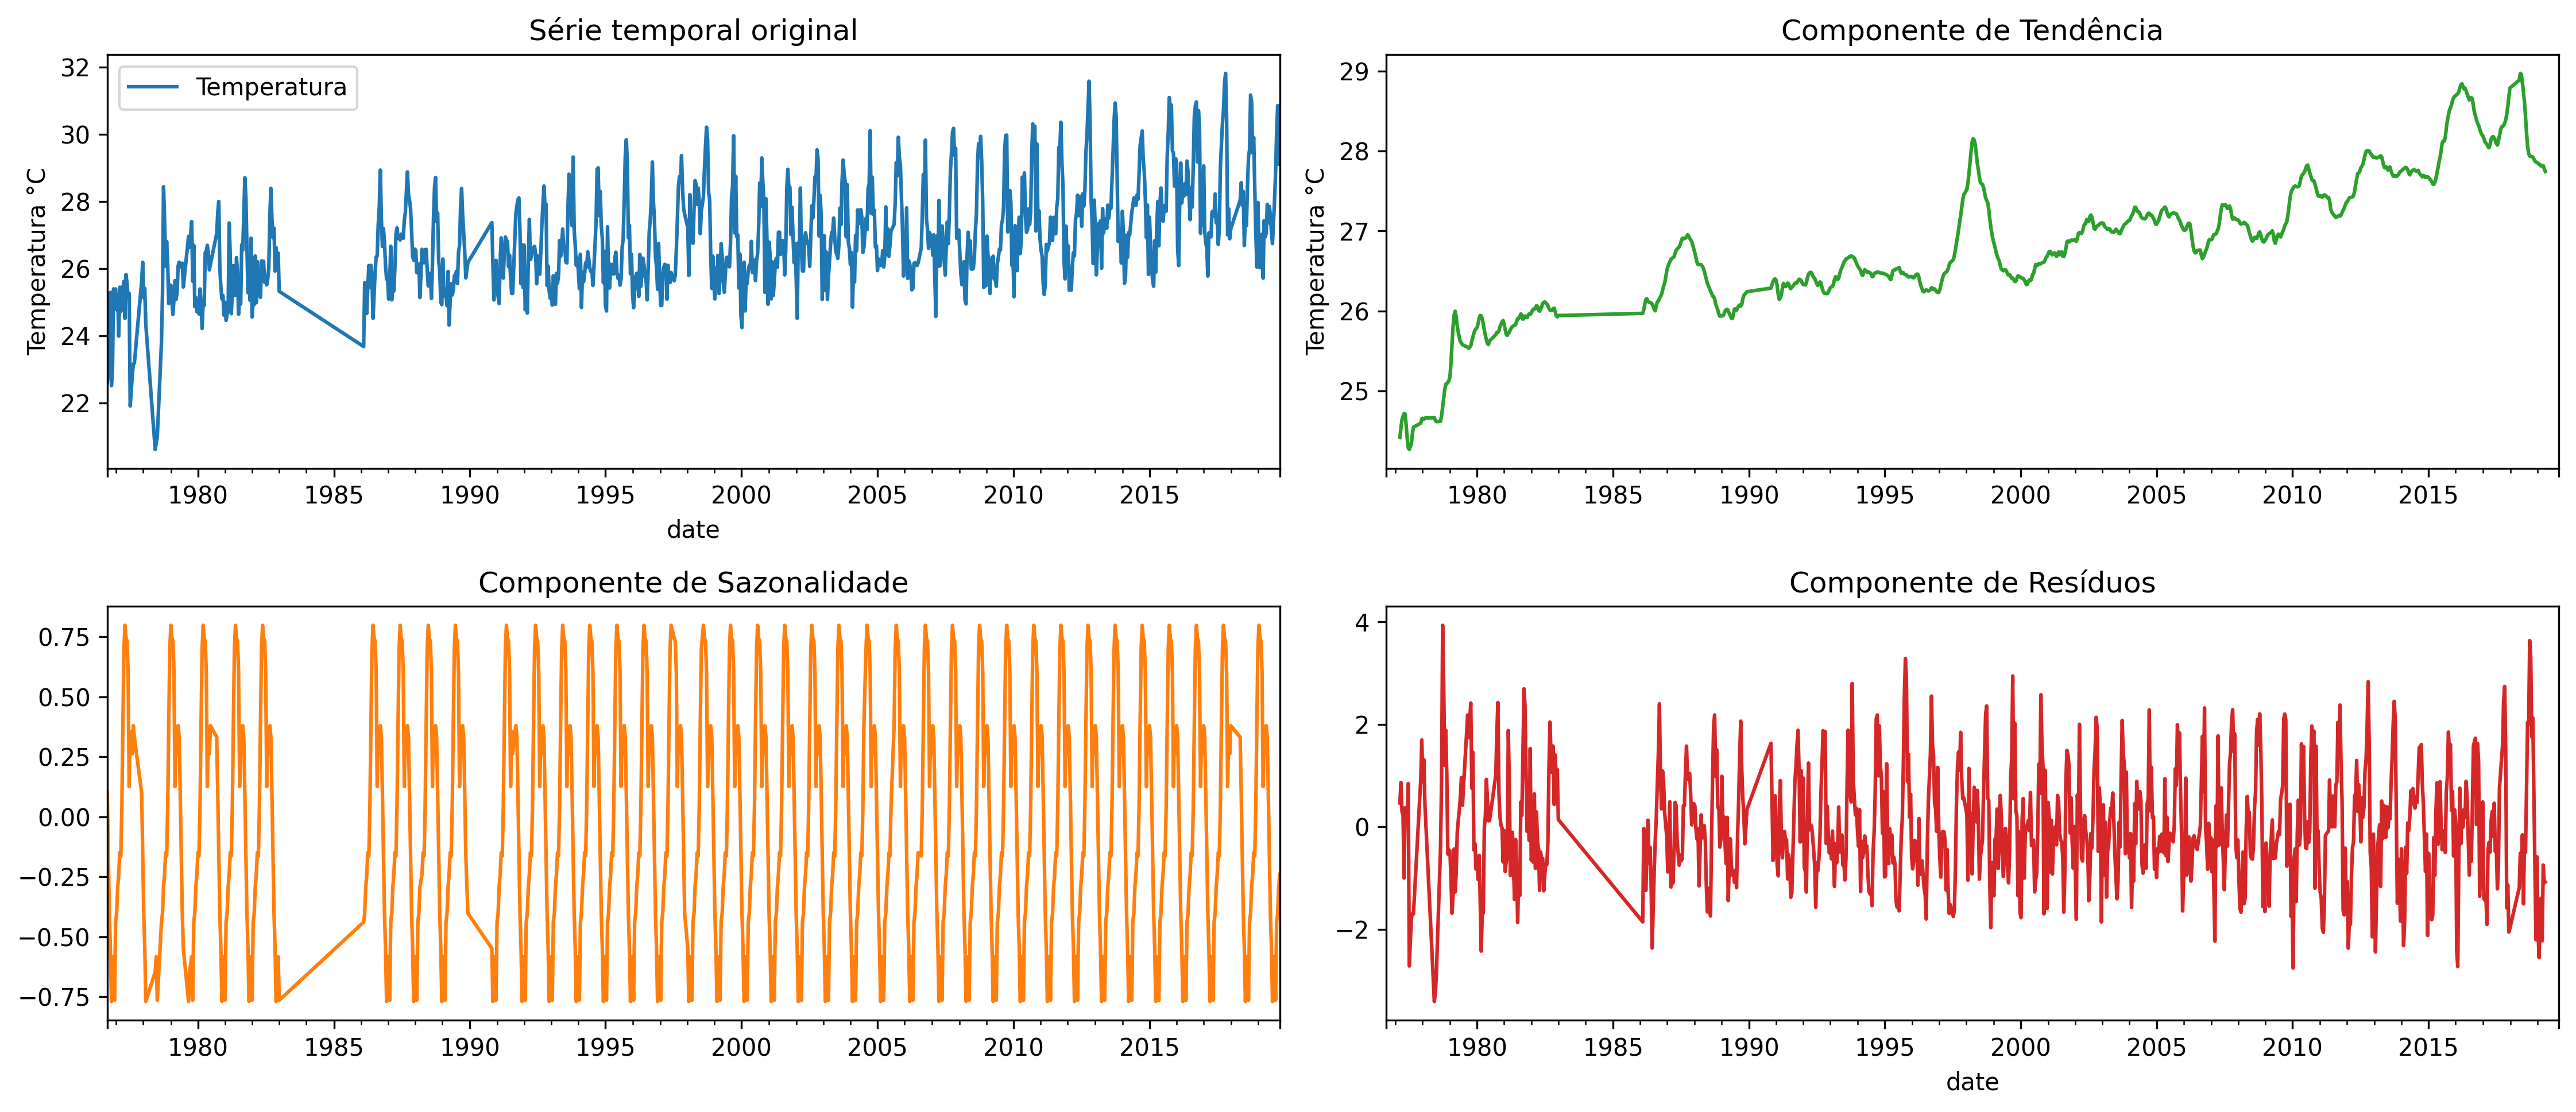
\includegraphics[width=0.9\textwidth]{figuras/decomposicao_82768.png}
    \label{fig:decomposicao_1}
\end{figure}

\begin{figure}[H]
    \centering
    \caption{Decomposição da série temporal da temperatura do ar para a estação automática localizada no município de Ariranha, no estado de São Paulo.}
    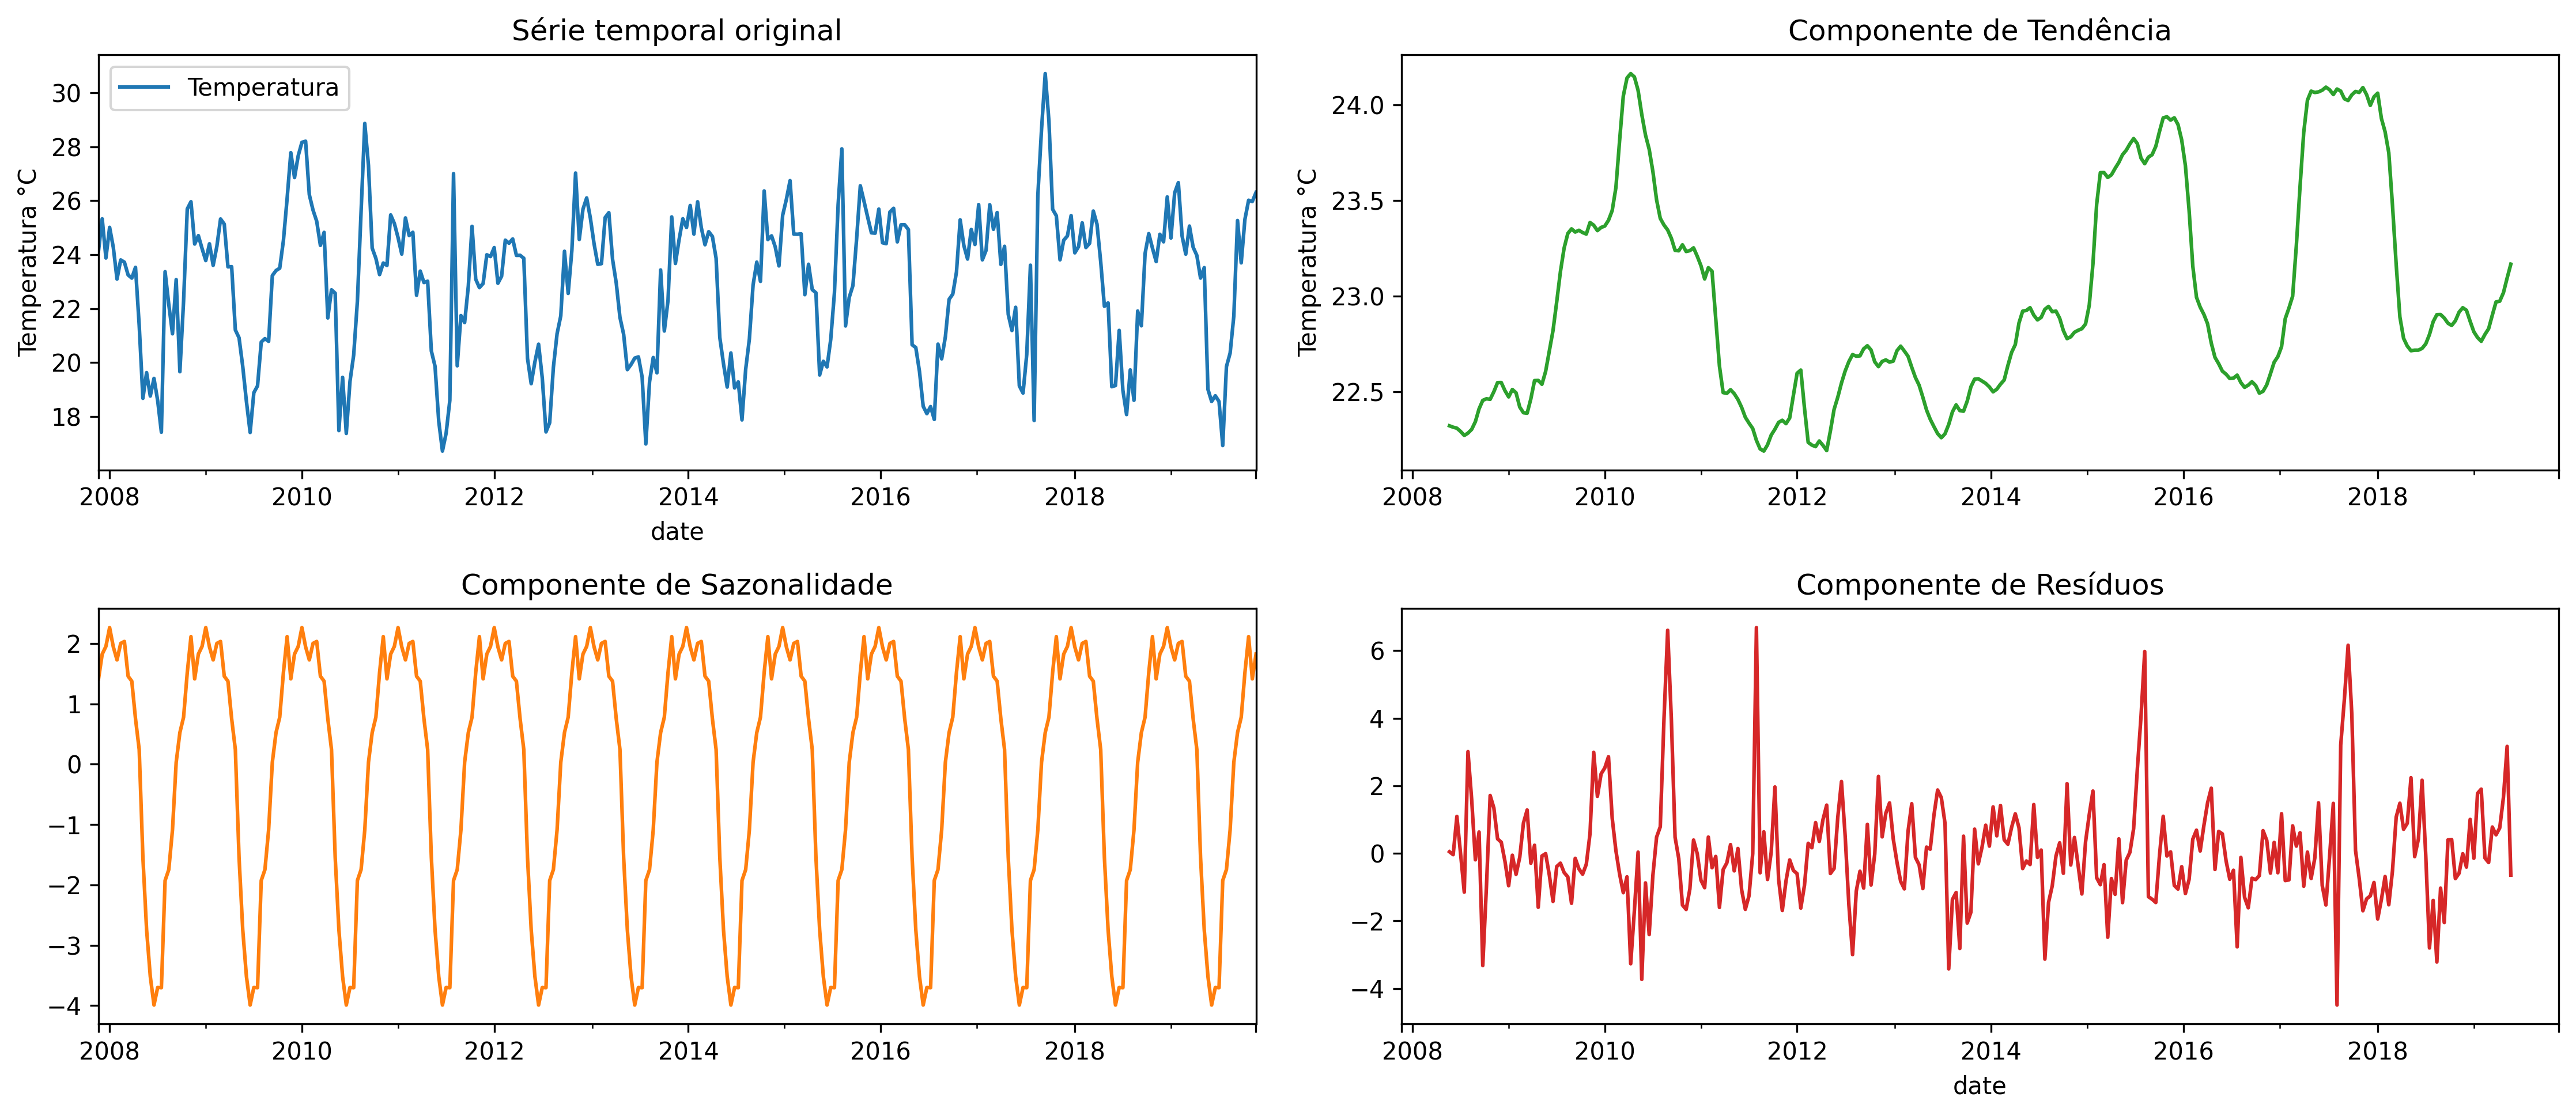
\includegraphics[width=0.9\textwidth]{figuras/decomposicao_A736.png}
    \label{fig:decomposicao_2}
\end{figure}

\begin{figure}[H]
    \centering
    \caption{Decomposição da série temporal da temperatura do ar para a estação automática localizada no município de Petrolina, no estado de Pernambuco.}
    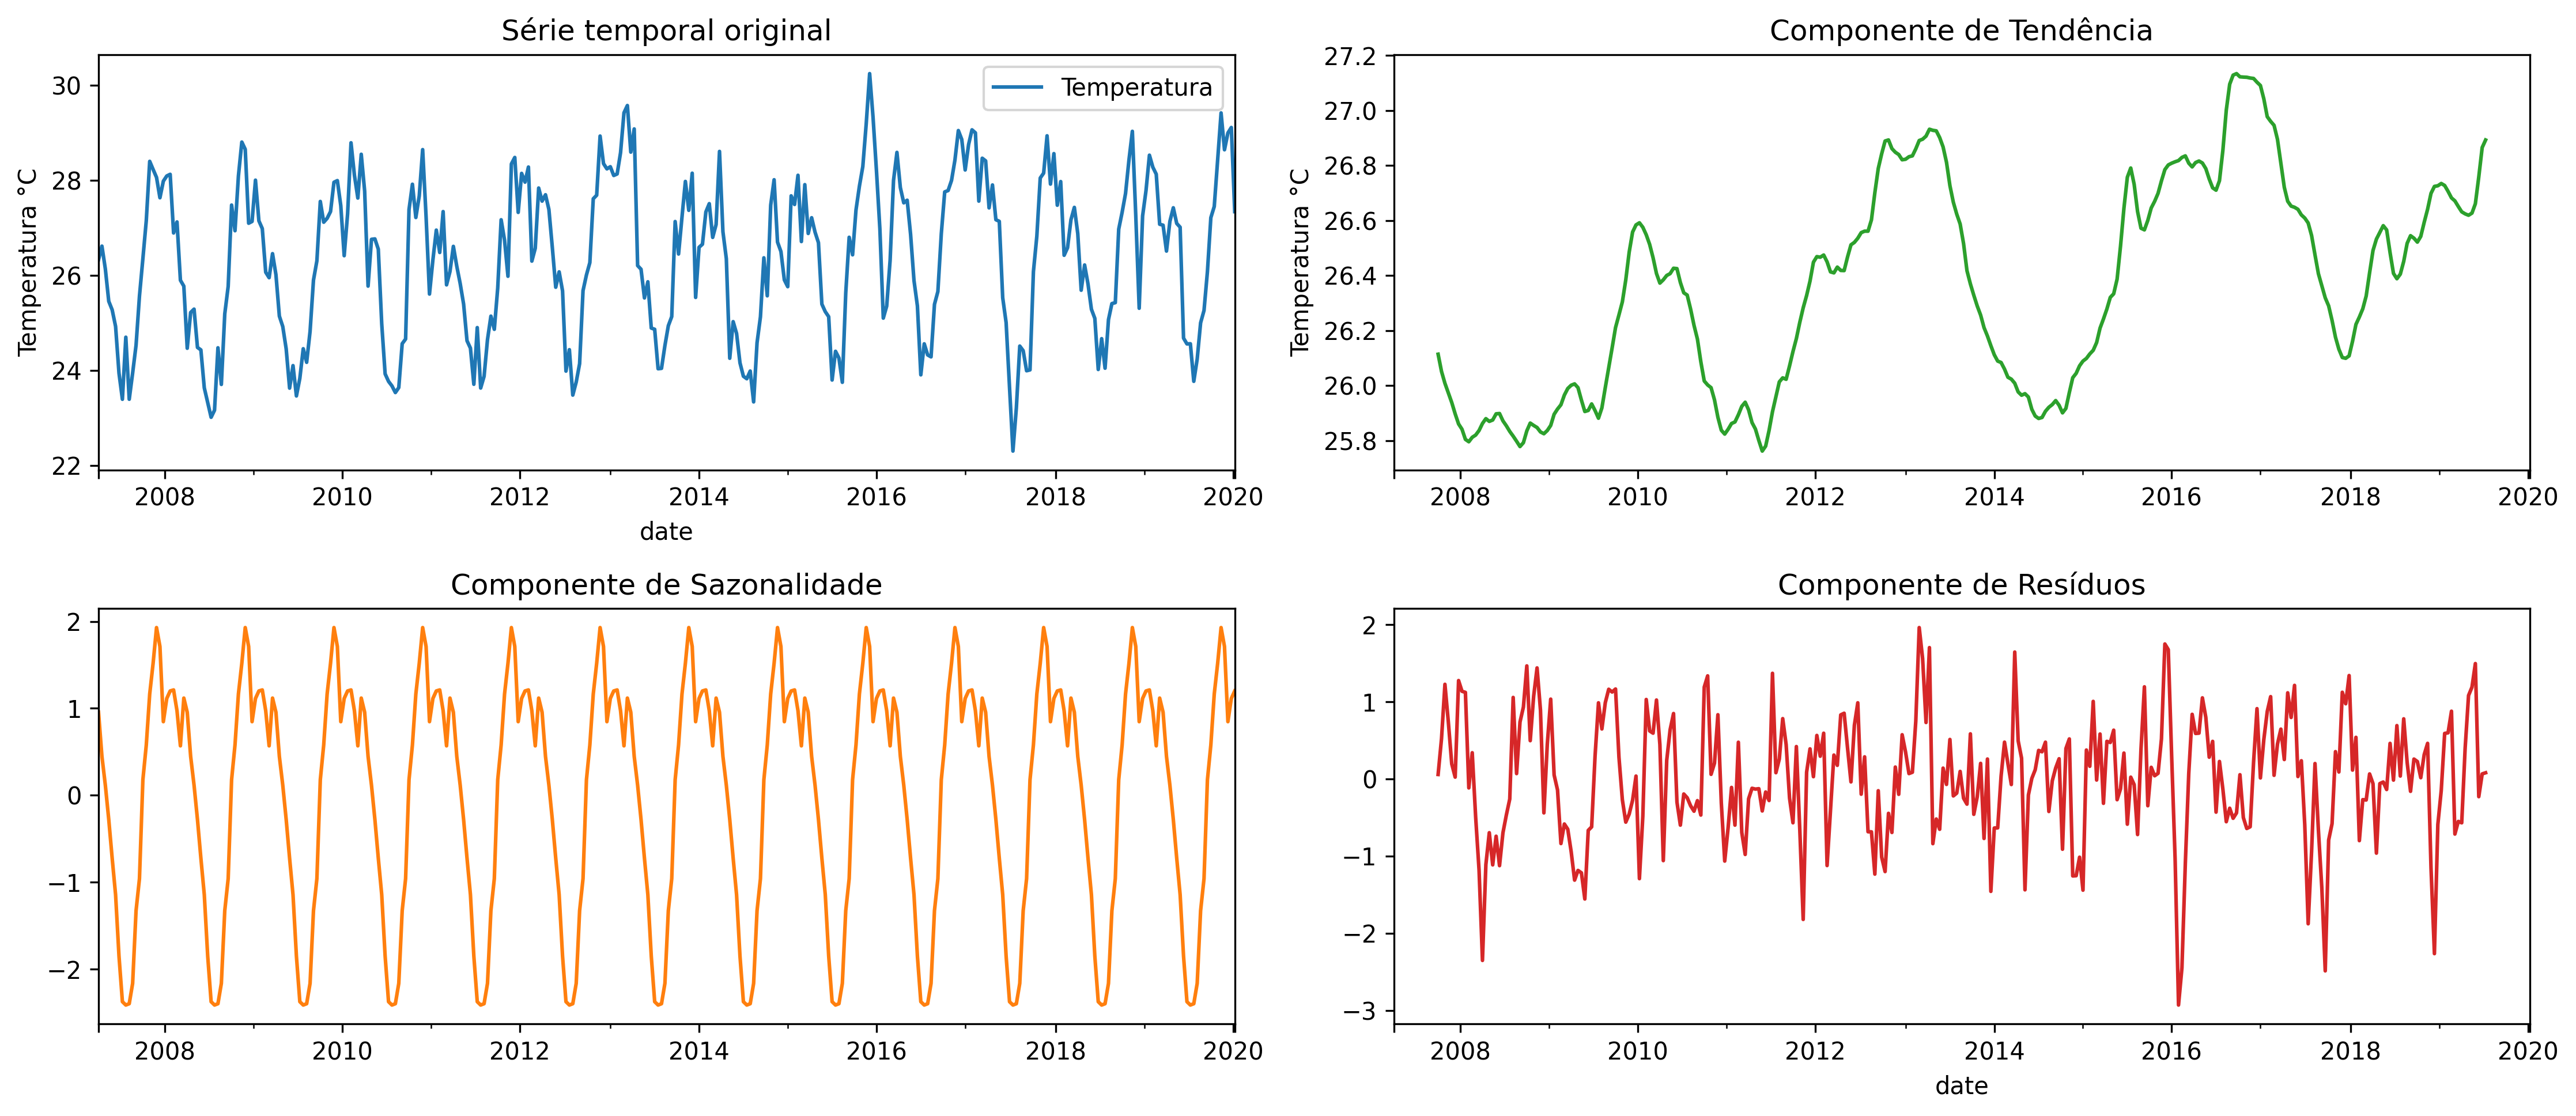
\includegraphics[width=0.9\textwidth]{figuras/decomposicao_712f3e11658051636f09732a60fb3c1b.png}
    \label{fig:decomposicao_3}
\end{figure}

Observando os componentes das séries temporais de exemplo, é possível observarmos uma forte tendencia anual nos dados de temperatura, confirmando a hipótese de que essa variável possui essa característica em seu comportamento.

\subsection{Autocorrelação das séries temporais}

Ao plotarmos a Autocorrelação para essas mesmas estações de exemplo, temos as figuras \ref{fig:correlacao_1}, \ref{fig:correlacao_2} e \ref{fig:correlacao_3}. 

\begin{figure}[H]
    \centering
    \caption{Autocorrelação da série temporal da temperatura do ar para a estação convencional localizada no município de Balsas, no estado do Maranhão.}
    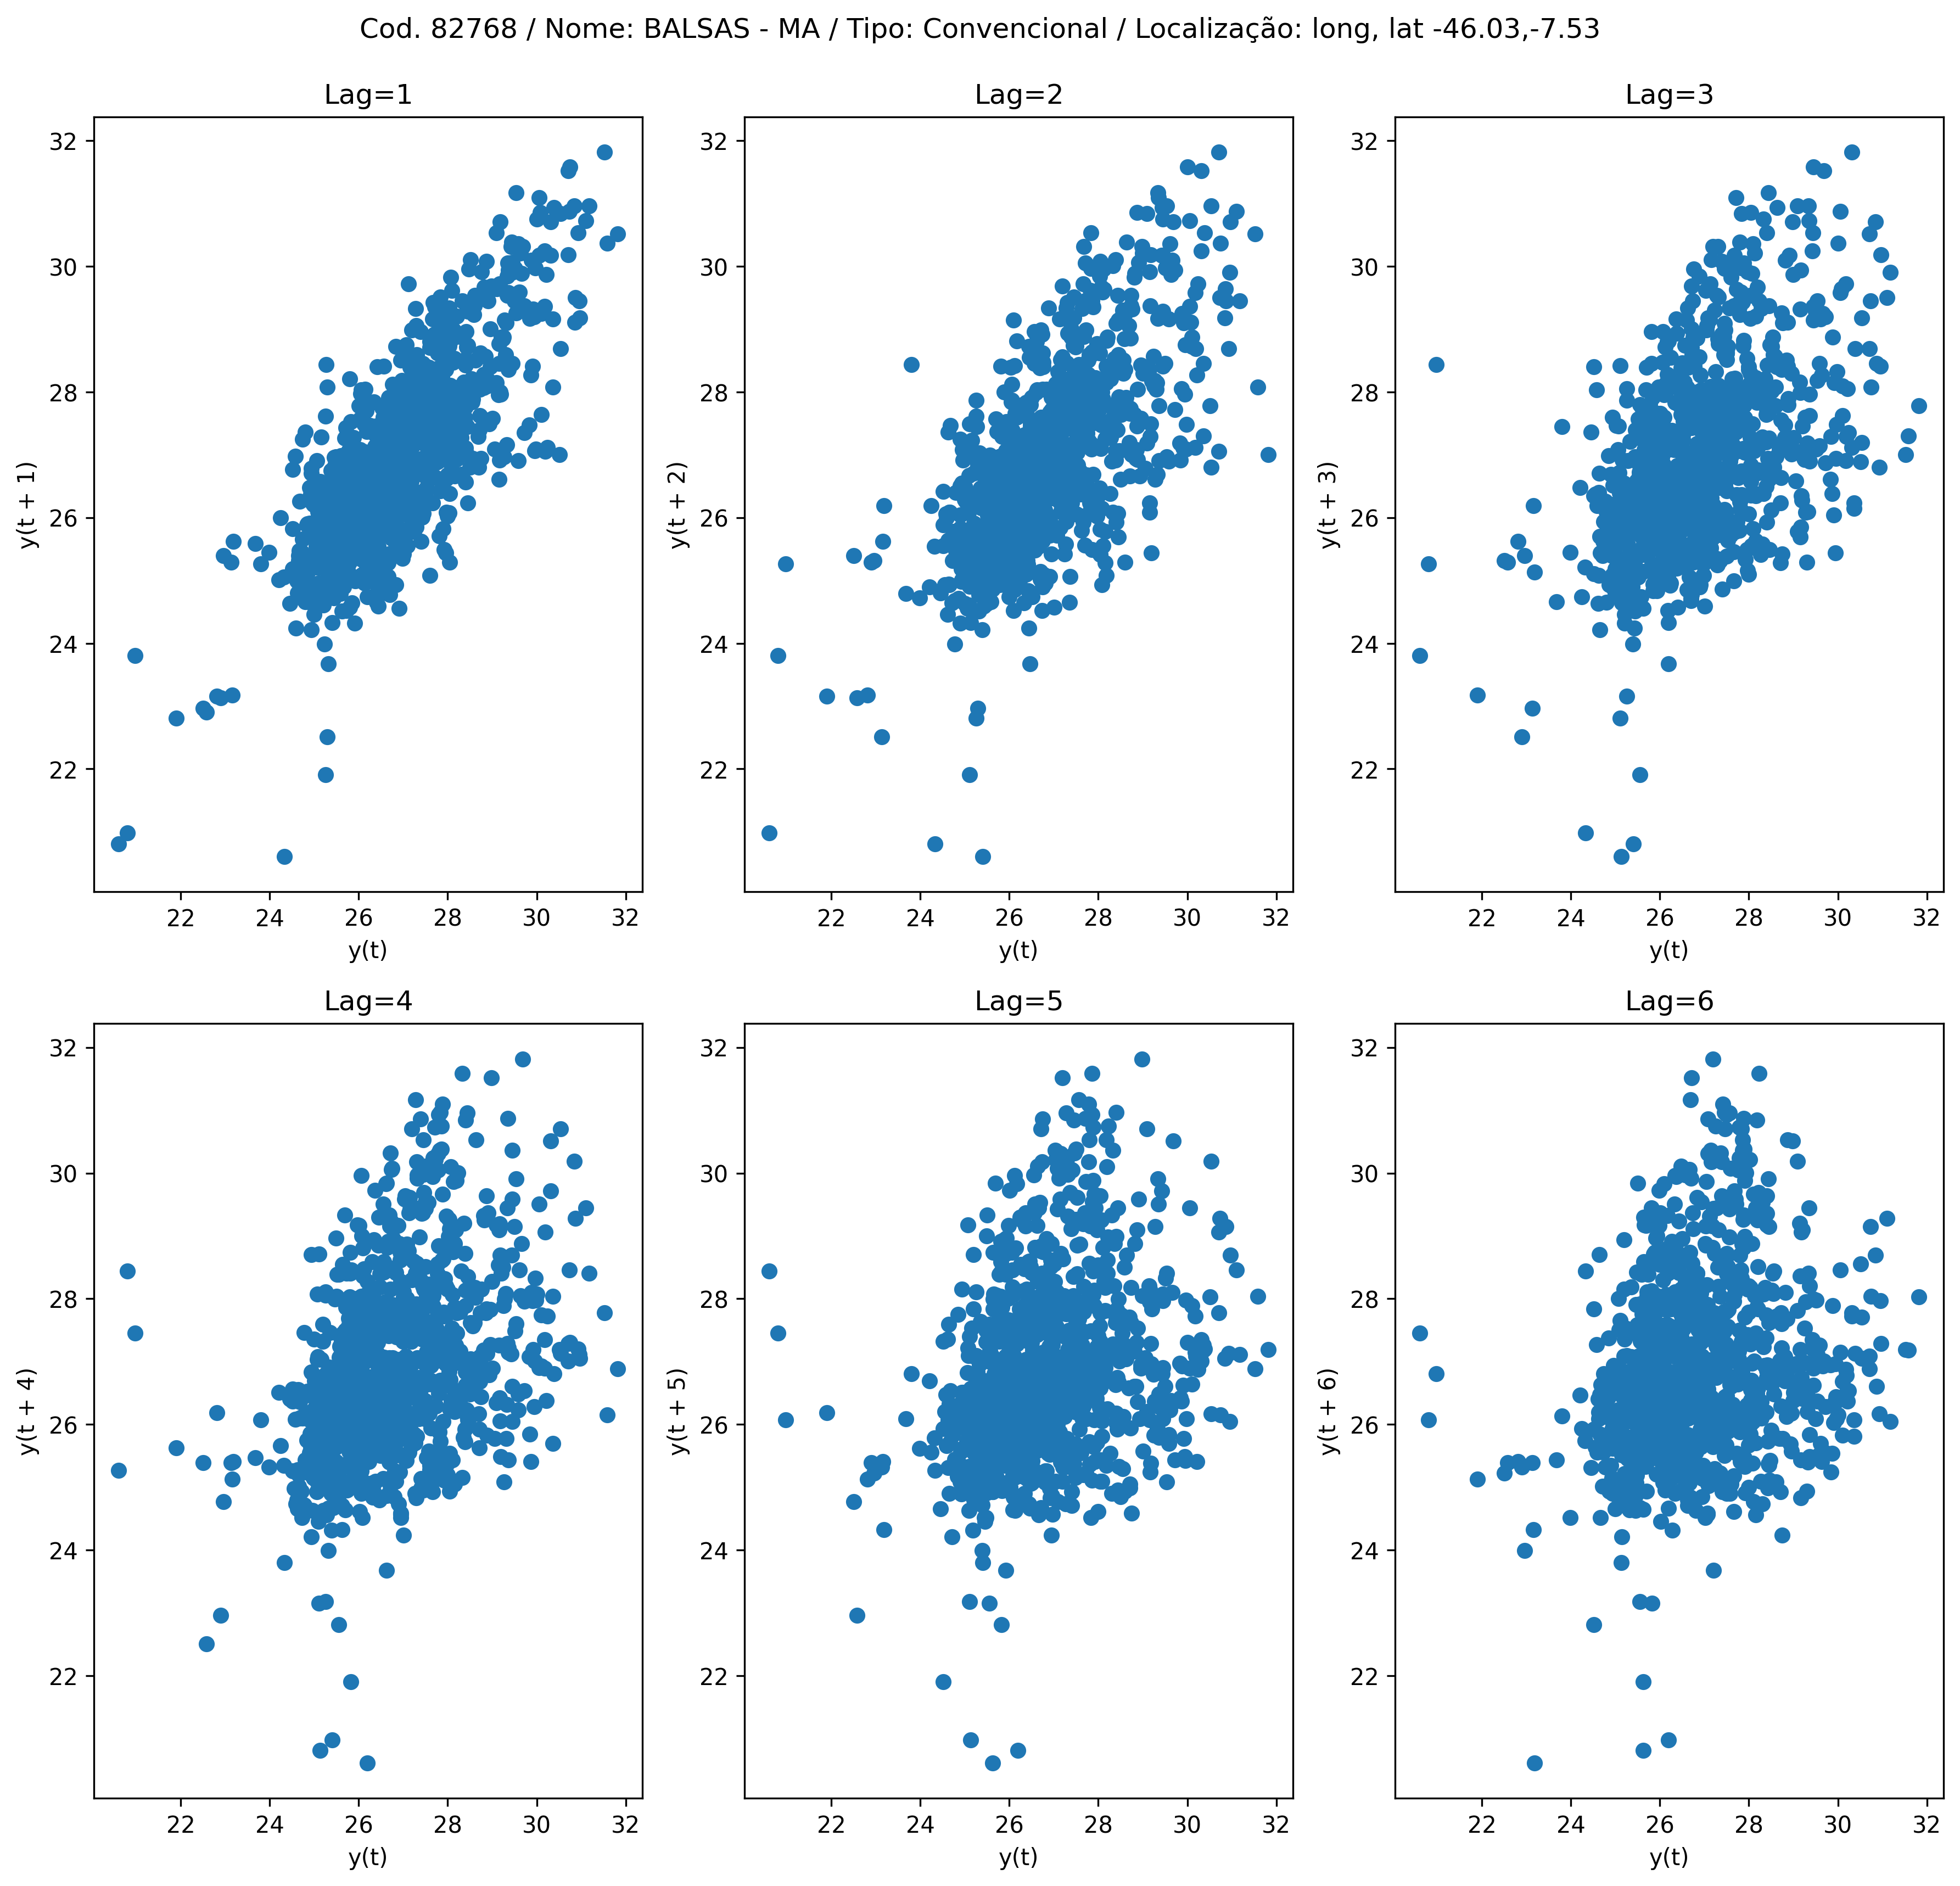
\includegraphics[width=0.9\textwidth]{figuras/correlacao_82768.png}
    \label{fig:correlacao_1}
\end{figure}

\begin{figure}[H]
    \centering
    \caption{Autocorrelação da série temporal da temperatura do ar para a estação automática localizada no município de Ariranha, no estado de São Paulo.}
    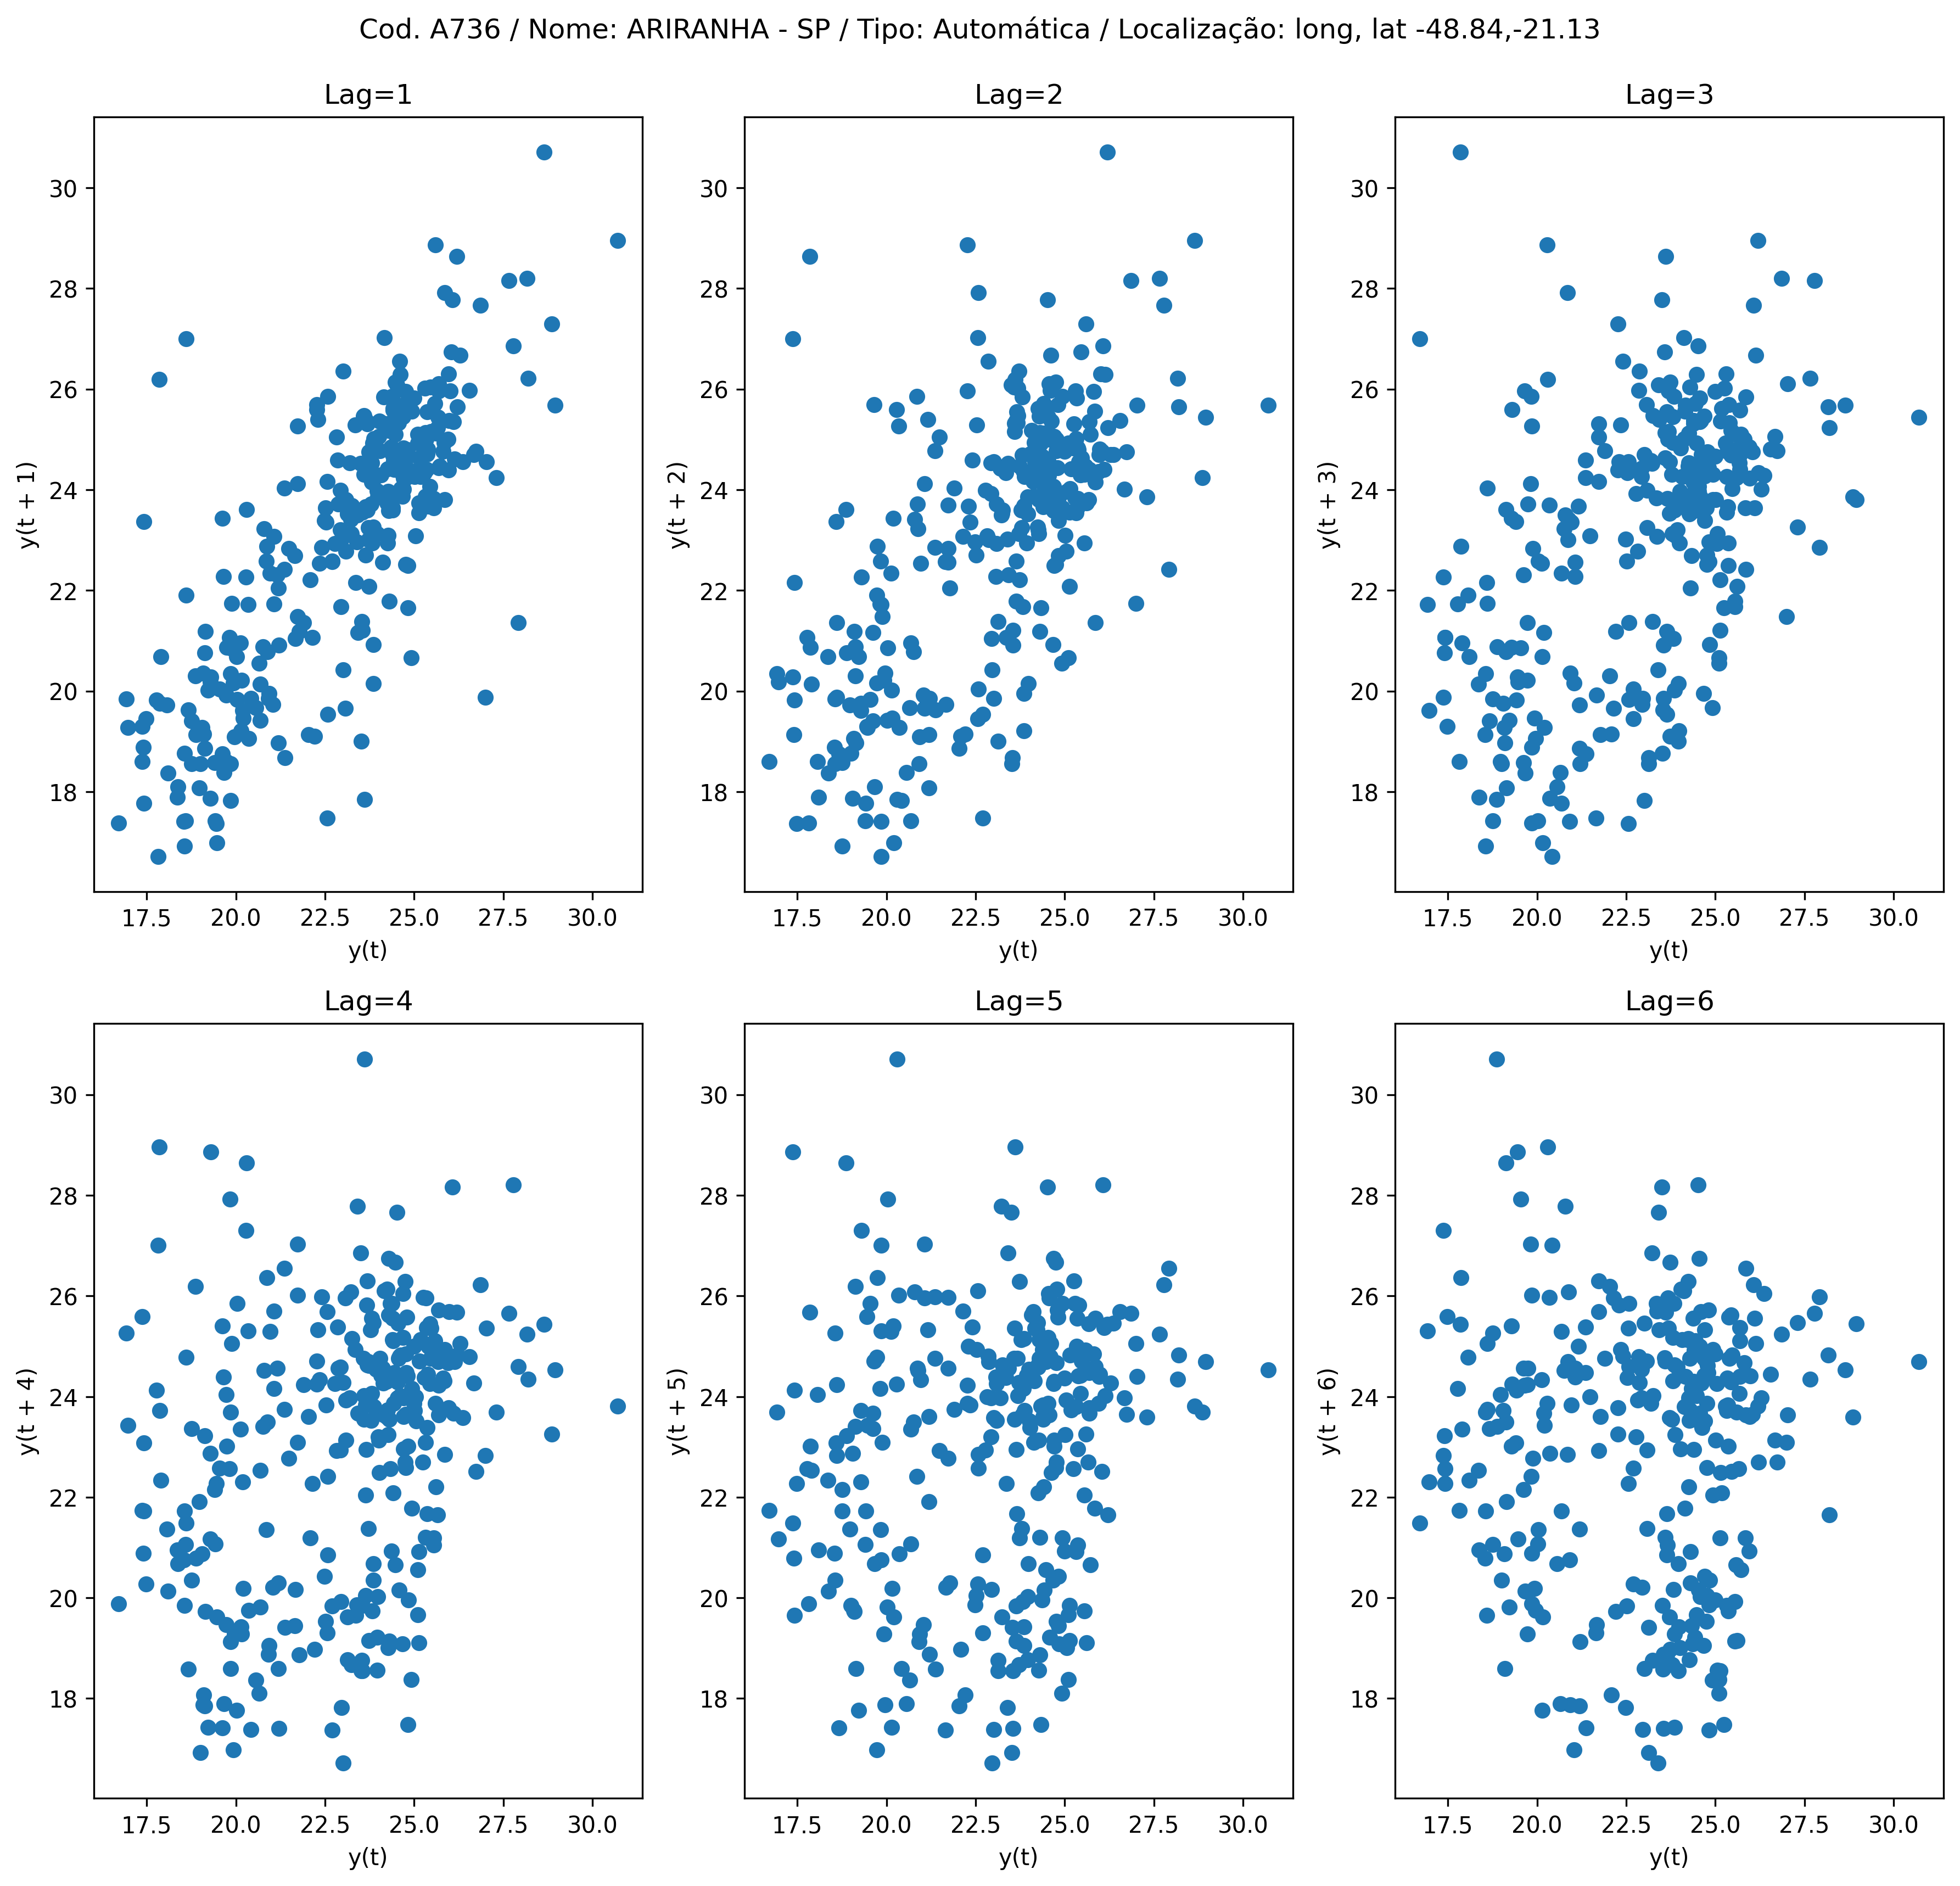
\includegraphics[width=0.9\textwidth]{figuras/correlacao_A736.png}
    \label{fig:correlacao_2}
\end{figure}

\begin{figure}[H]
    \centering
    \caption{Autocorrelação da série temporal da temperatura do ar para a estação automática localizada no município de Petrolina, no estado de Pernambuco.}
    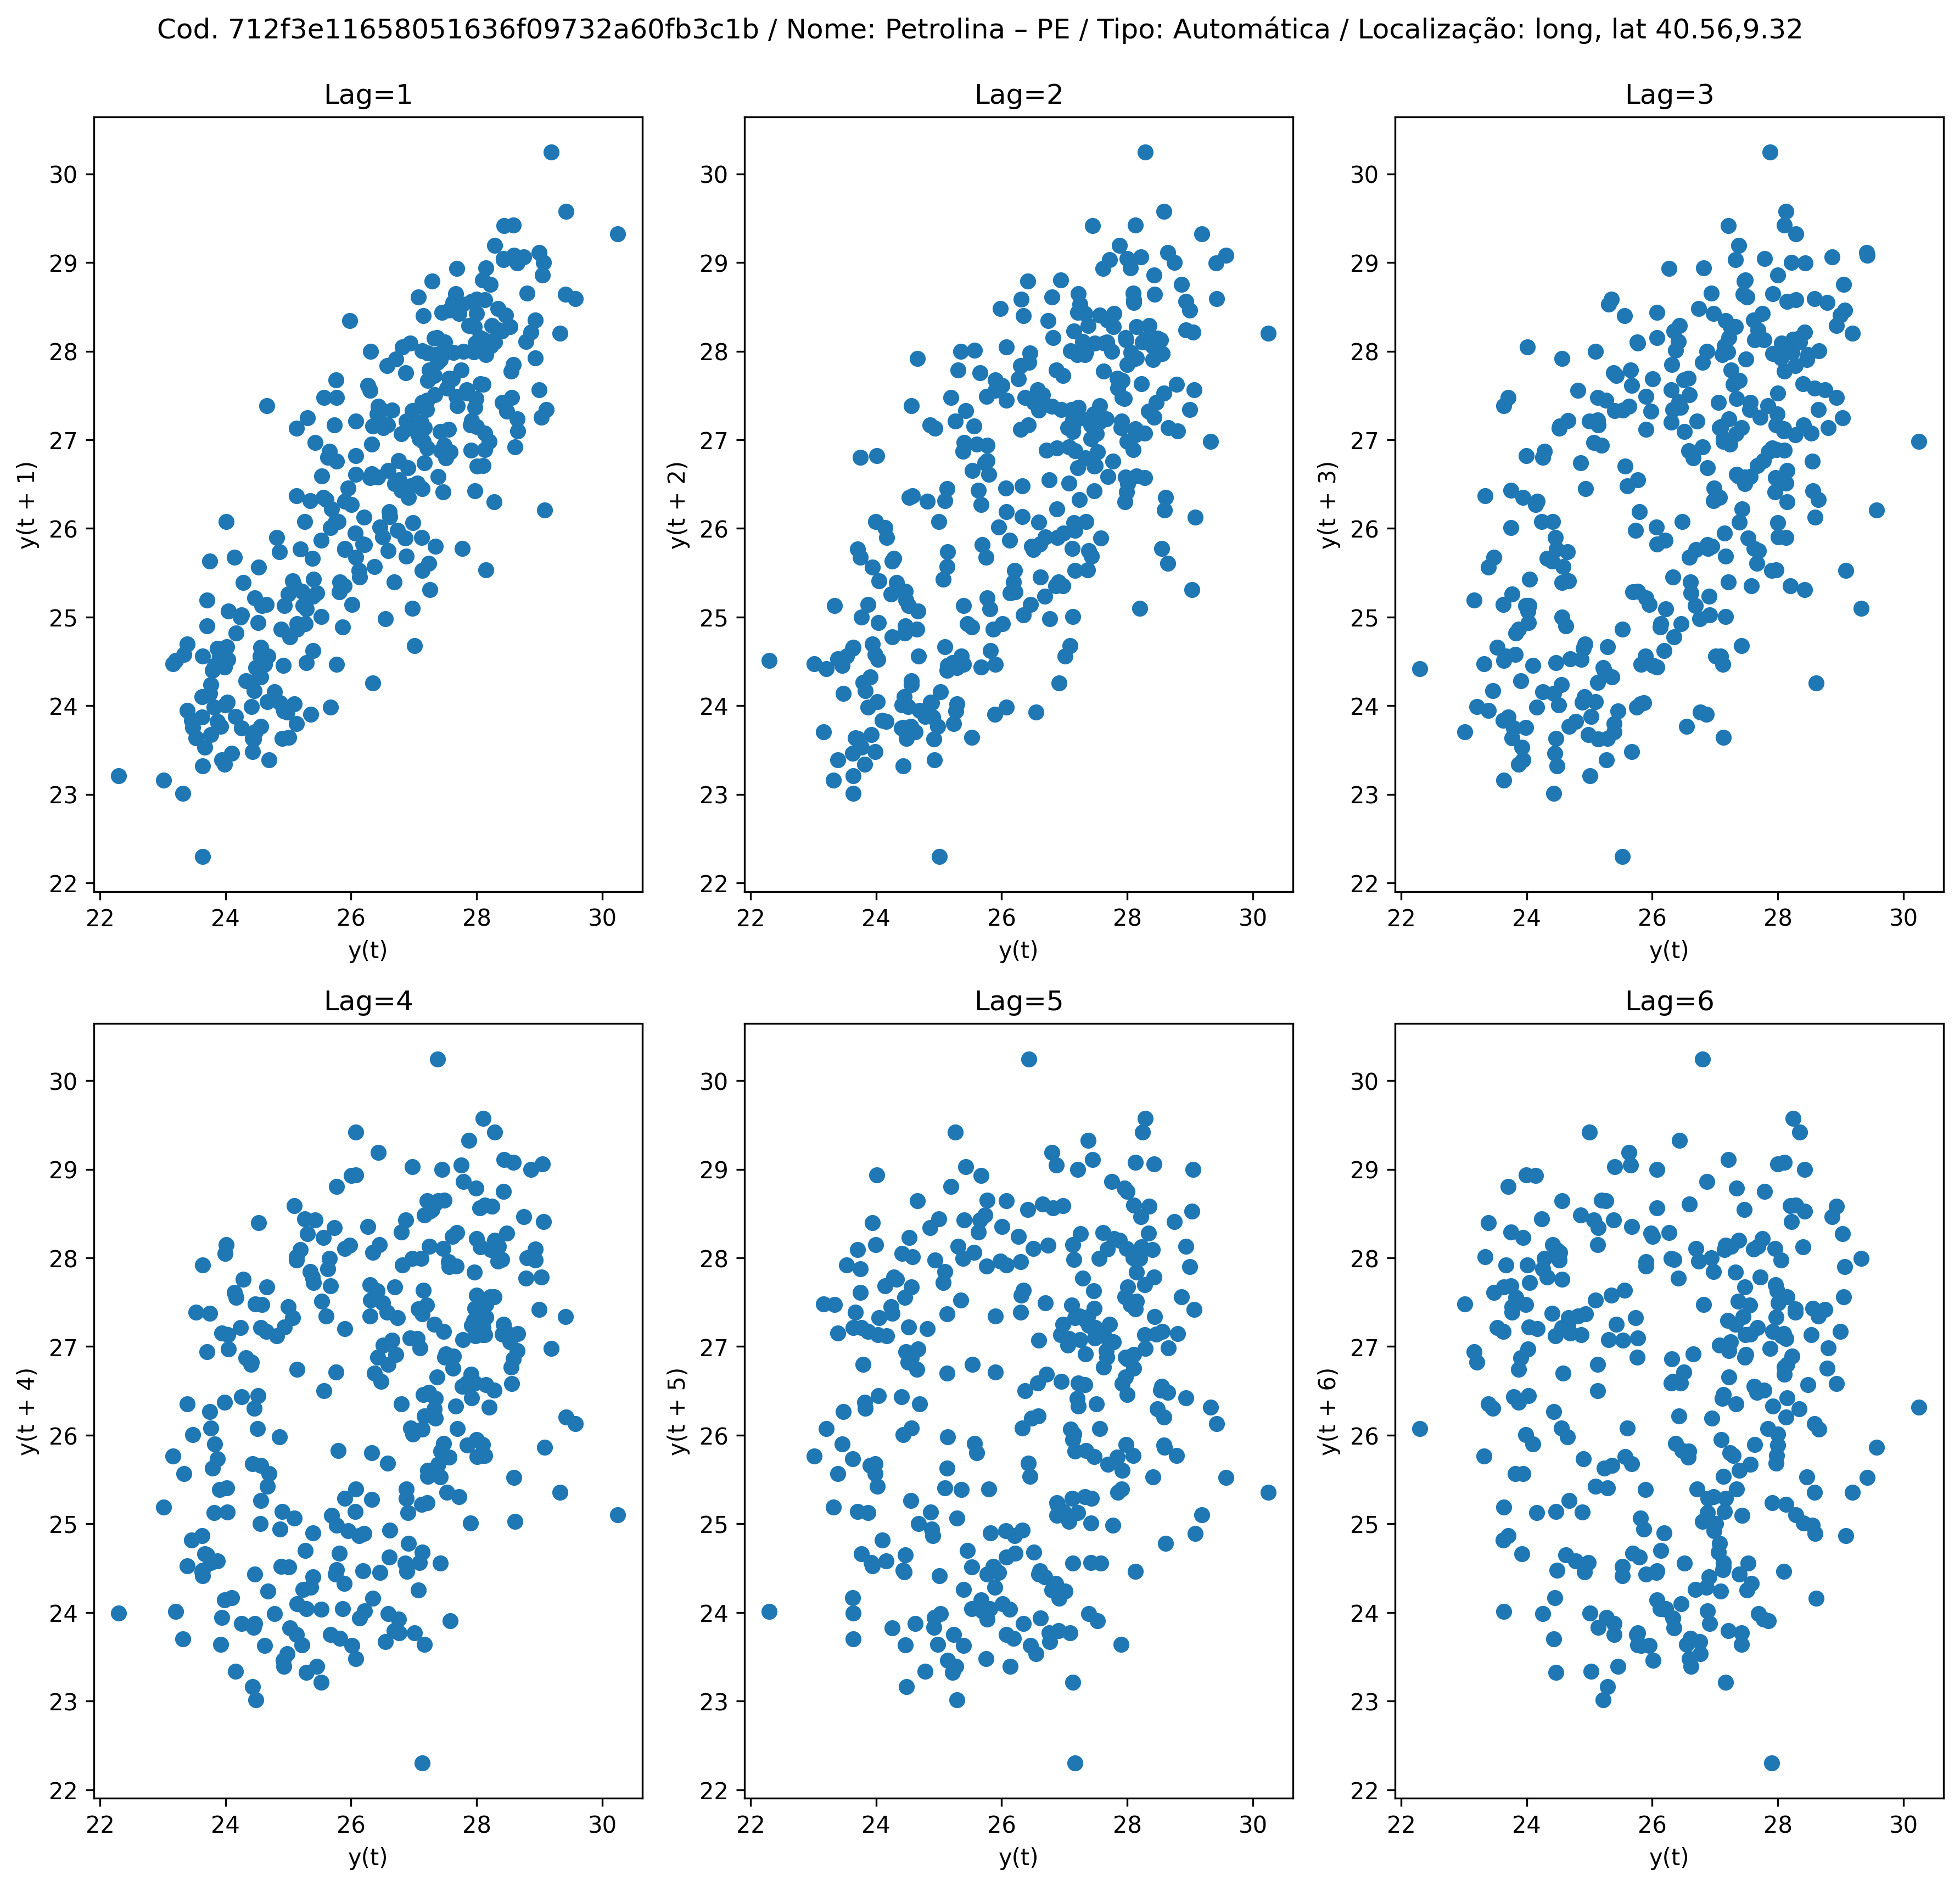
\includegraphics[width=0.9\textwidth]{figuras/correlacao_712f3e11658051636f09732a60fb3c1b.png}
    \label{fig:correlacao_3}
\end{figure}

Verificando os gráficos de autocorrelação, podemos verificar que não há uma alta autocorrelação nas estações de exemplo, por isso há a necessidade de se utilizar um modelo auto-arima para identificação do melhor modelo de forma automática.

\subsection{Verificando a estacionalidade}

A maioria dos modelos de previsão de séries temporais exigem que os dados sejam estacionários. Uma série temporal é considerada estacionária se suas propriedades estatísticas, como média, variância e covariância permanecerem constantes ao longo do tempo \cite{box2011time}. Para verificarmos se as séries que estamos trabalhando são estacionárias, utilizamos o teste de Dickey-Fuller aumentado \cite{said1984testing}. 

Apresentamos o resultado da verificação da estacionalidade das estações utilizadas como exemplo nas Figuras \ref{fig:estacionalidade_seria_original_1}, \ref{fig:estacionalidade_seria_original_2} e \ref{fig:estacionalidade_seria_original_3}.

\begin{figure}[H]
    \centering
    \caption{Teste de estacionalidade da série temporal da temperatura do ar para a estação convencional localizada no município de Balsas, no estado do Maranhão.}
    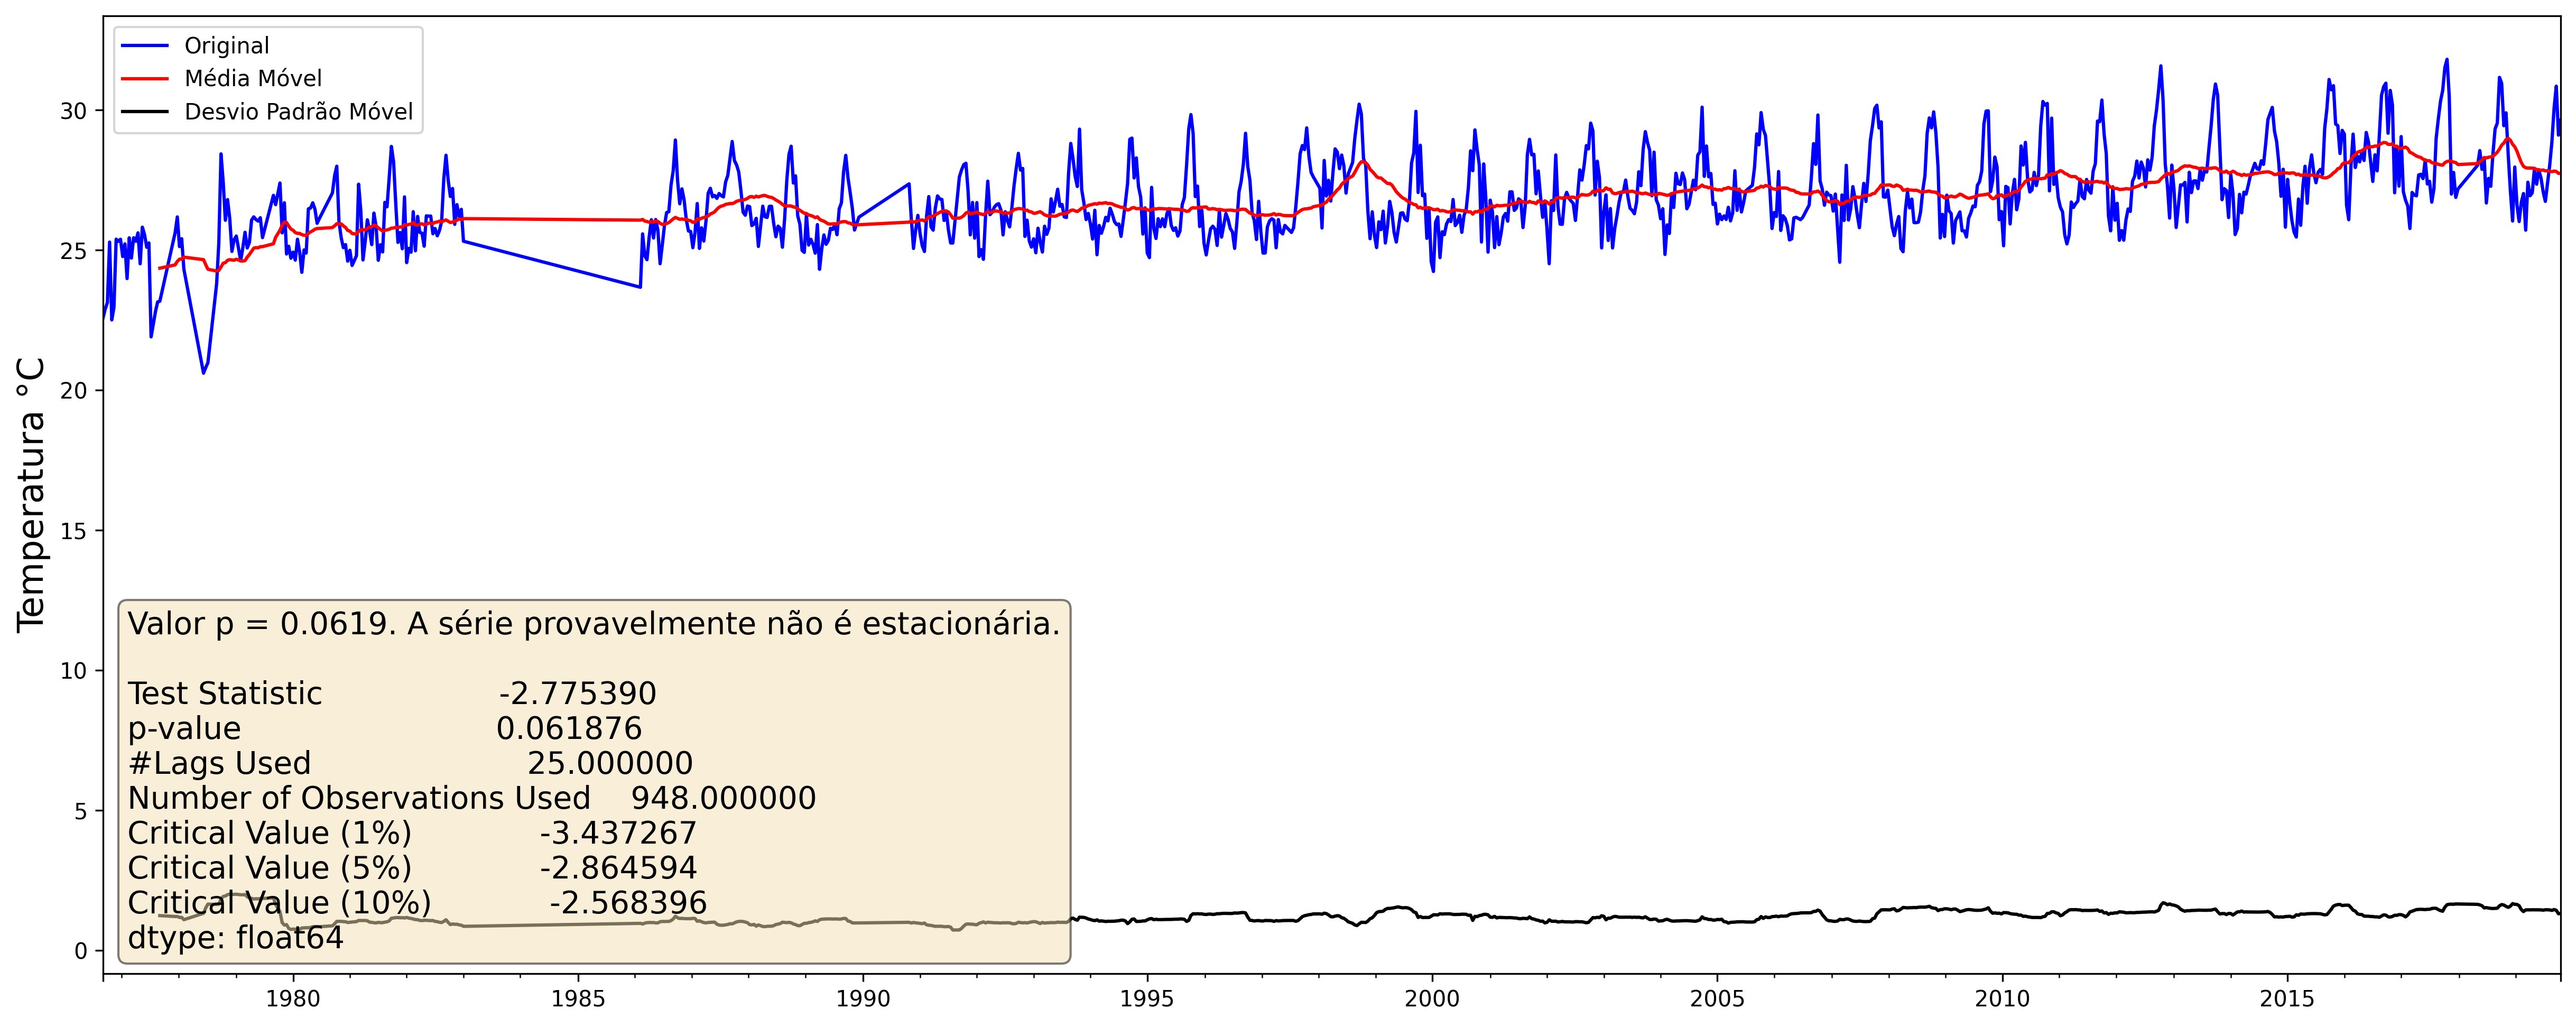
\includegraphics[width=0.9\textwidth]{figuras/dickey_fuller_raw_82768.png}
    \label{fig:estacionalidade_seria_original_1}
\end{figure}

\begin{figure}[H]
    \centering
    \caption{Teste de estacionalidade da série temporal da temperatura do ar para a estação automática localizada no município de Ariranha, no estado de São Paulo.}
    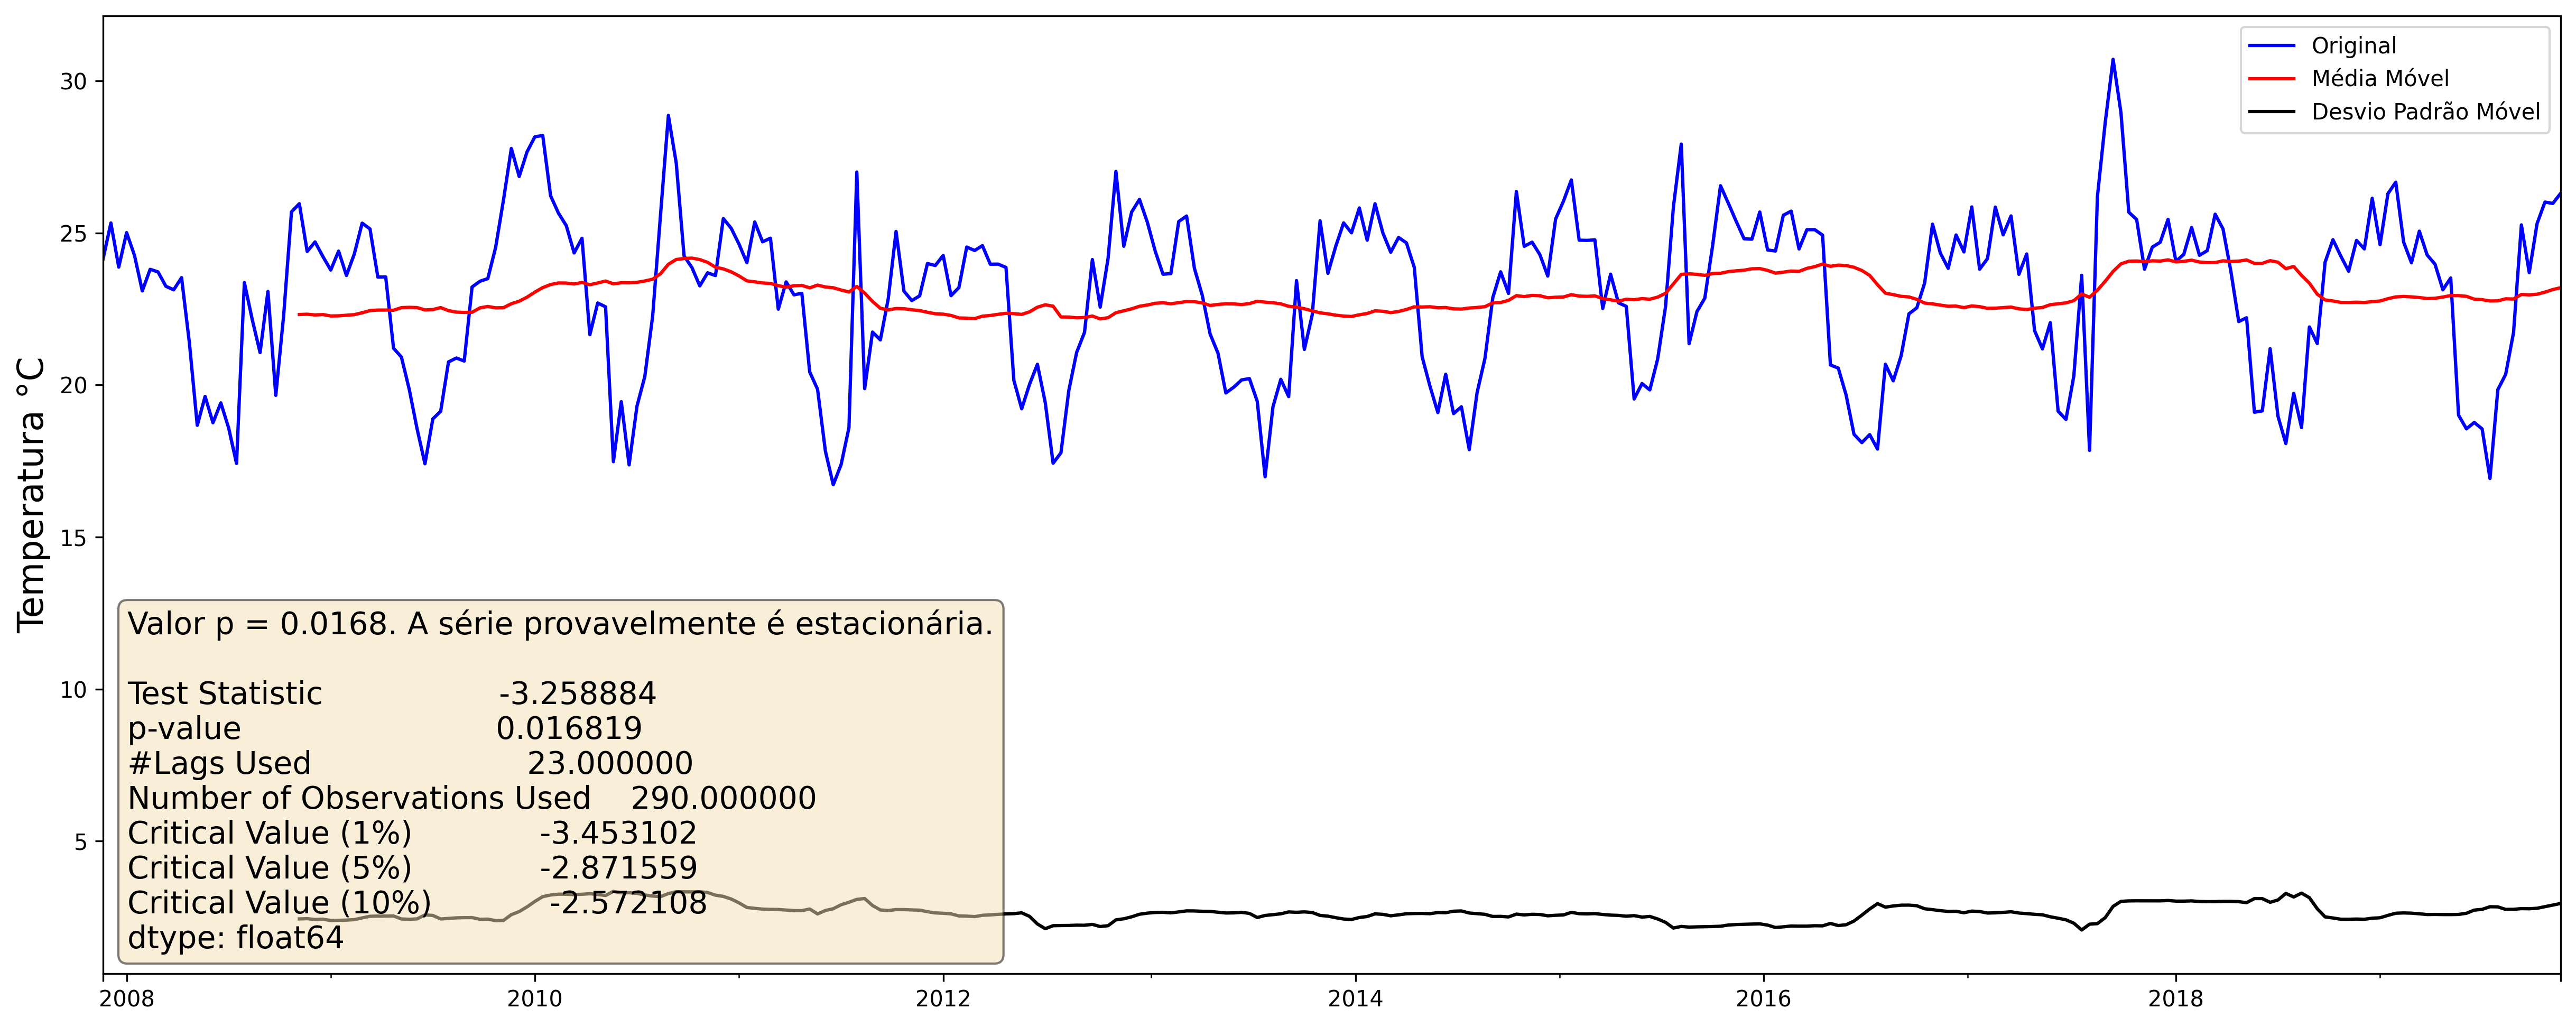
\includegraphics[width=0.9\textwidth]{figuras/dickey_fuller_raw_A736.png}
    \label{fig:estacionalidade_seria_original_2}
\end{figure}

\begin{figure}[H]
    \centering
    \caption{Teste de estacionalidade da série temporal da temperatura do ar para a estação automática localizada no município de Petrolina, no estado de Pernambuco.}
    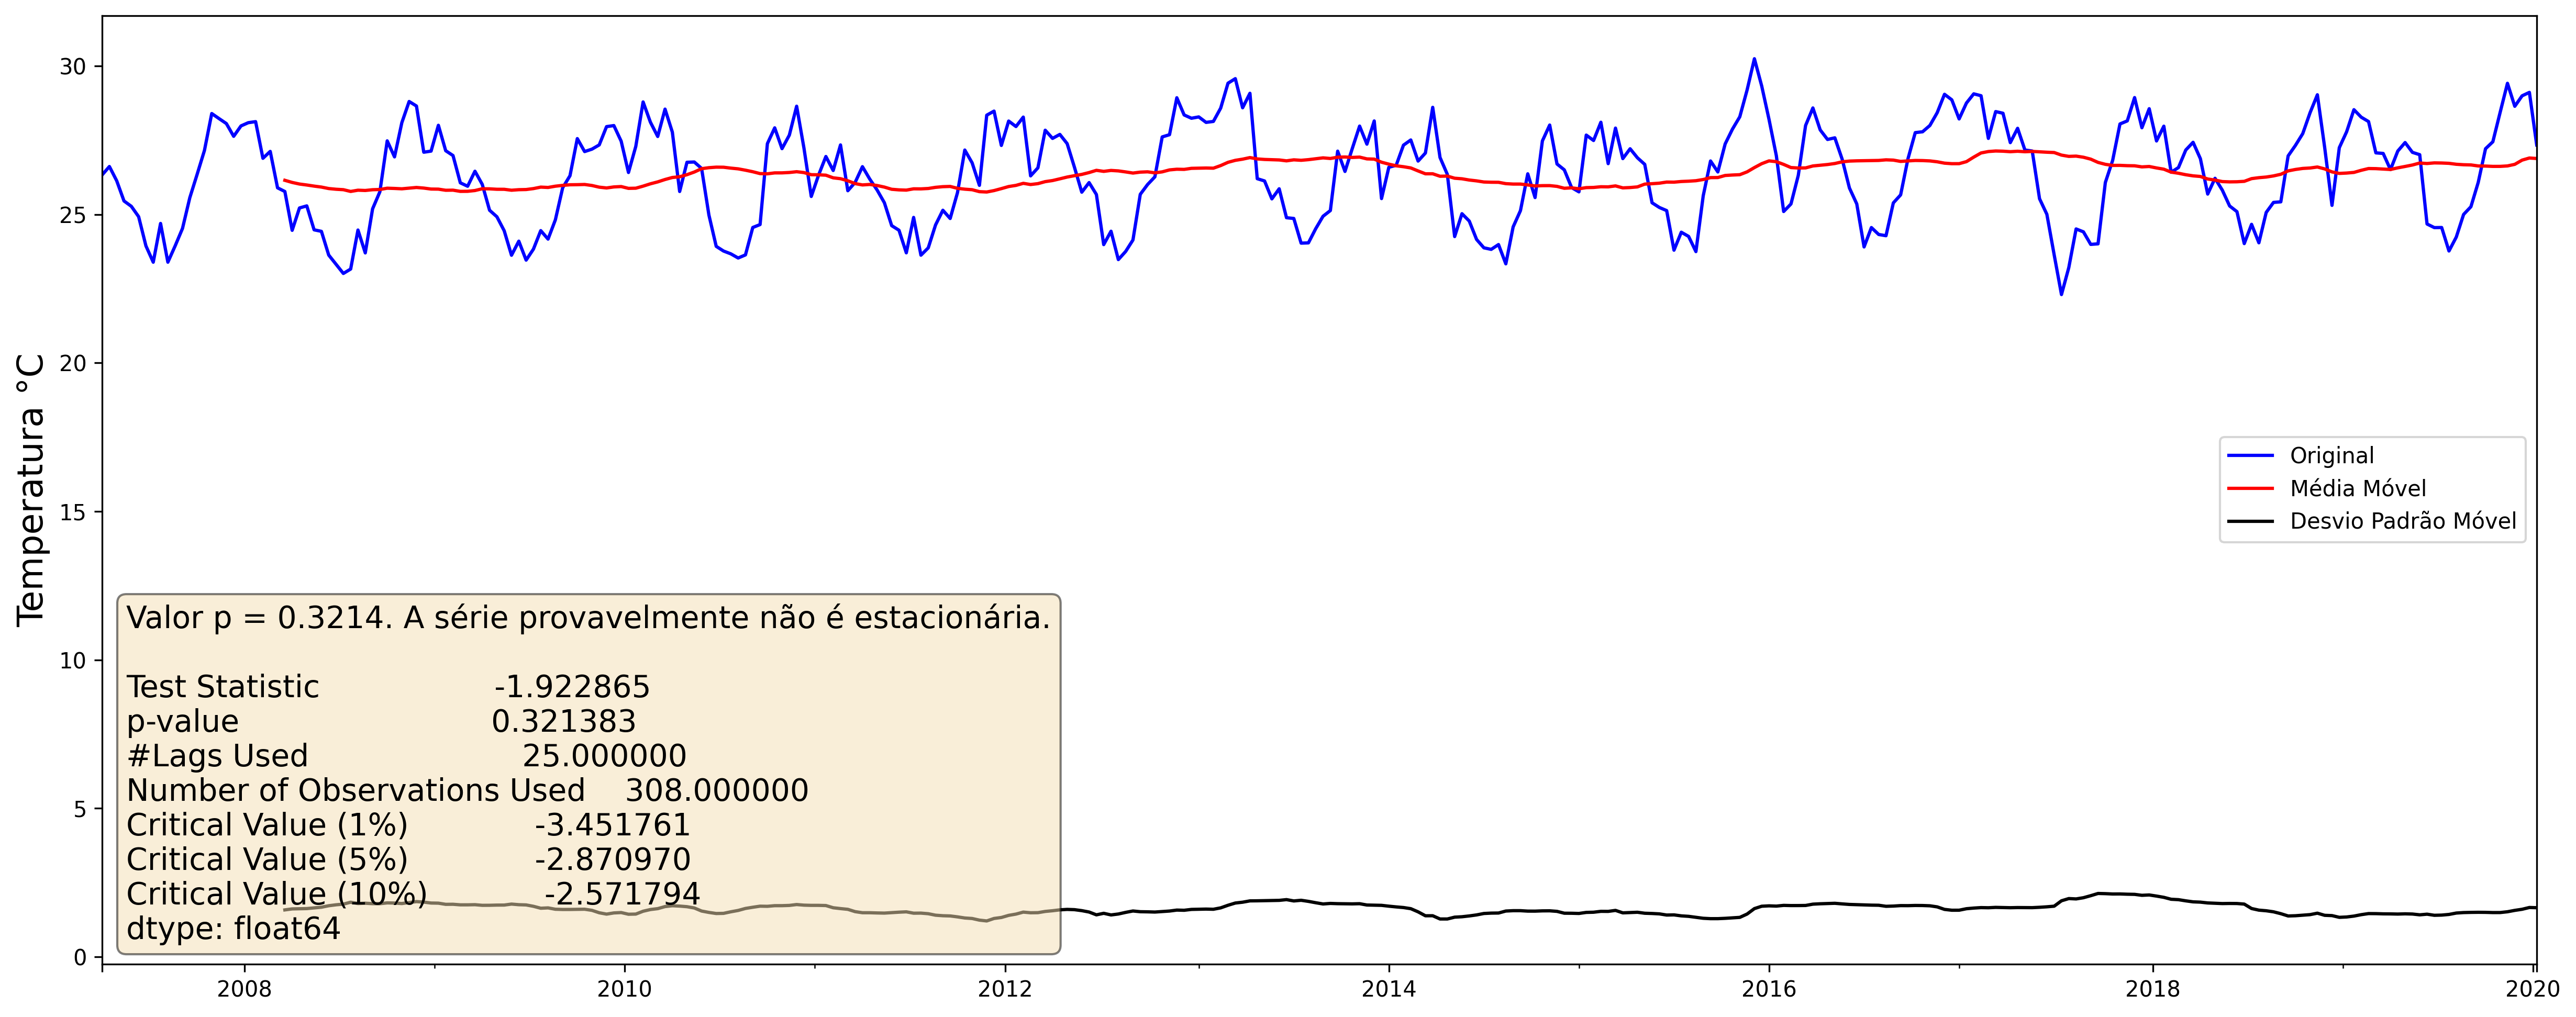
\includegraphics[width=0.9\textwidth]{figuras/dickey_fuller_raw_712f3e11658051636f09732a60fb3c1b.png}
    \label{fig:estacionalidade_seria_original_3}
\end{figure}

Pelo valor de p ser maior que 0,05, podemos afirmar que a primeira e a última série não são estacionarias, enquanto a segunda série, com o valor de p próximo de ~0,01, indica que a série é estacionária. Para garantirmos que todas as séries utilizadas por nosso modelo sejam estacionárias, aplicamos uma diferenciação de primeira ordem com o objetivo de torna-las todas séries estacionarias. 

Após o processo de diferenciação, realizamos novamente o teste de Dickey-Fuller aumentado e obtivemos os resultados apresentados das figuras \ref{fig:estacionalidade_seria_diferenciada_1}, \ref{fig:estacionalidade_seria_diferenciada_2} e \ref{fig:estacionalidade_seria_diferenciada_3}.  

\begin{figure}[H]
    \centering
    \caption{Teste de estacionalidade da série temporal diferenciada da temperatura do ar para a estação convencional localizada no município de Balsas, no estado do Maranhão.}
    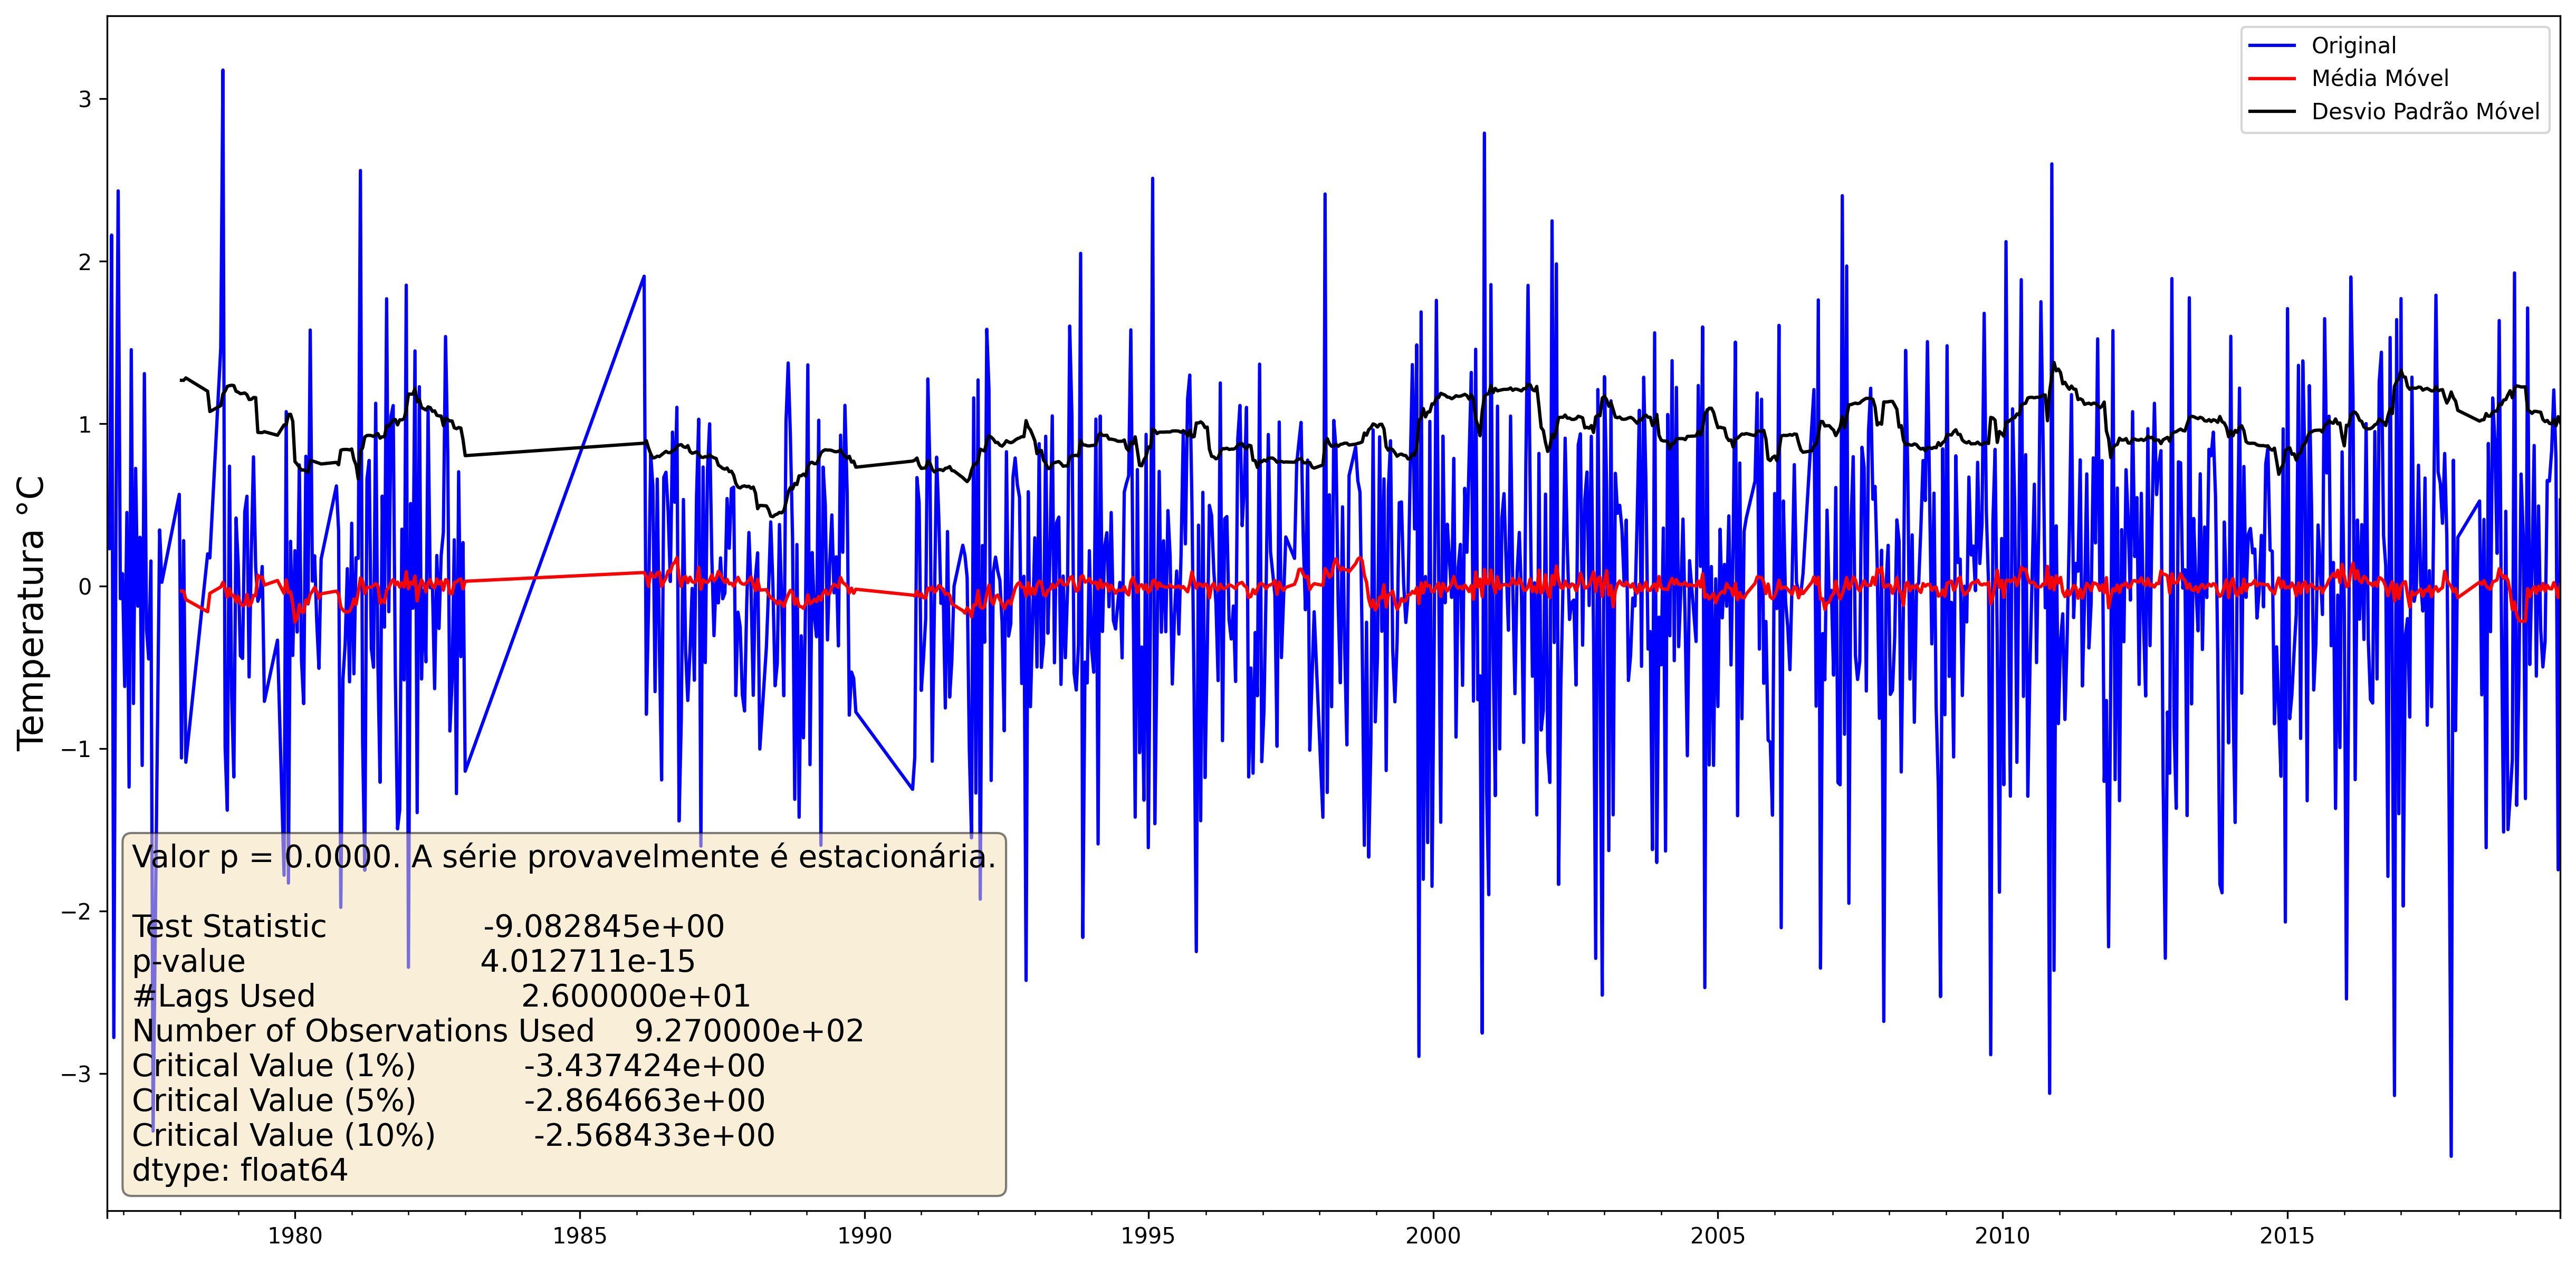
\includegraphics[width=0.9\textwidth]{figuras/dickey_fuller_diff_82768.png}
    \label{fig:estacionalidade_seria_diferenciada_1}
\end{figure}

\begin{figure}[H]
    \centering
    \caption{Teste de estacionalidade da série temporal diferenciada da temperatura do ar para a estação automática localizada no município de Ariranha, no estado de São Paulo.}
    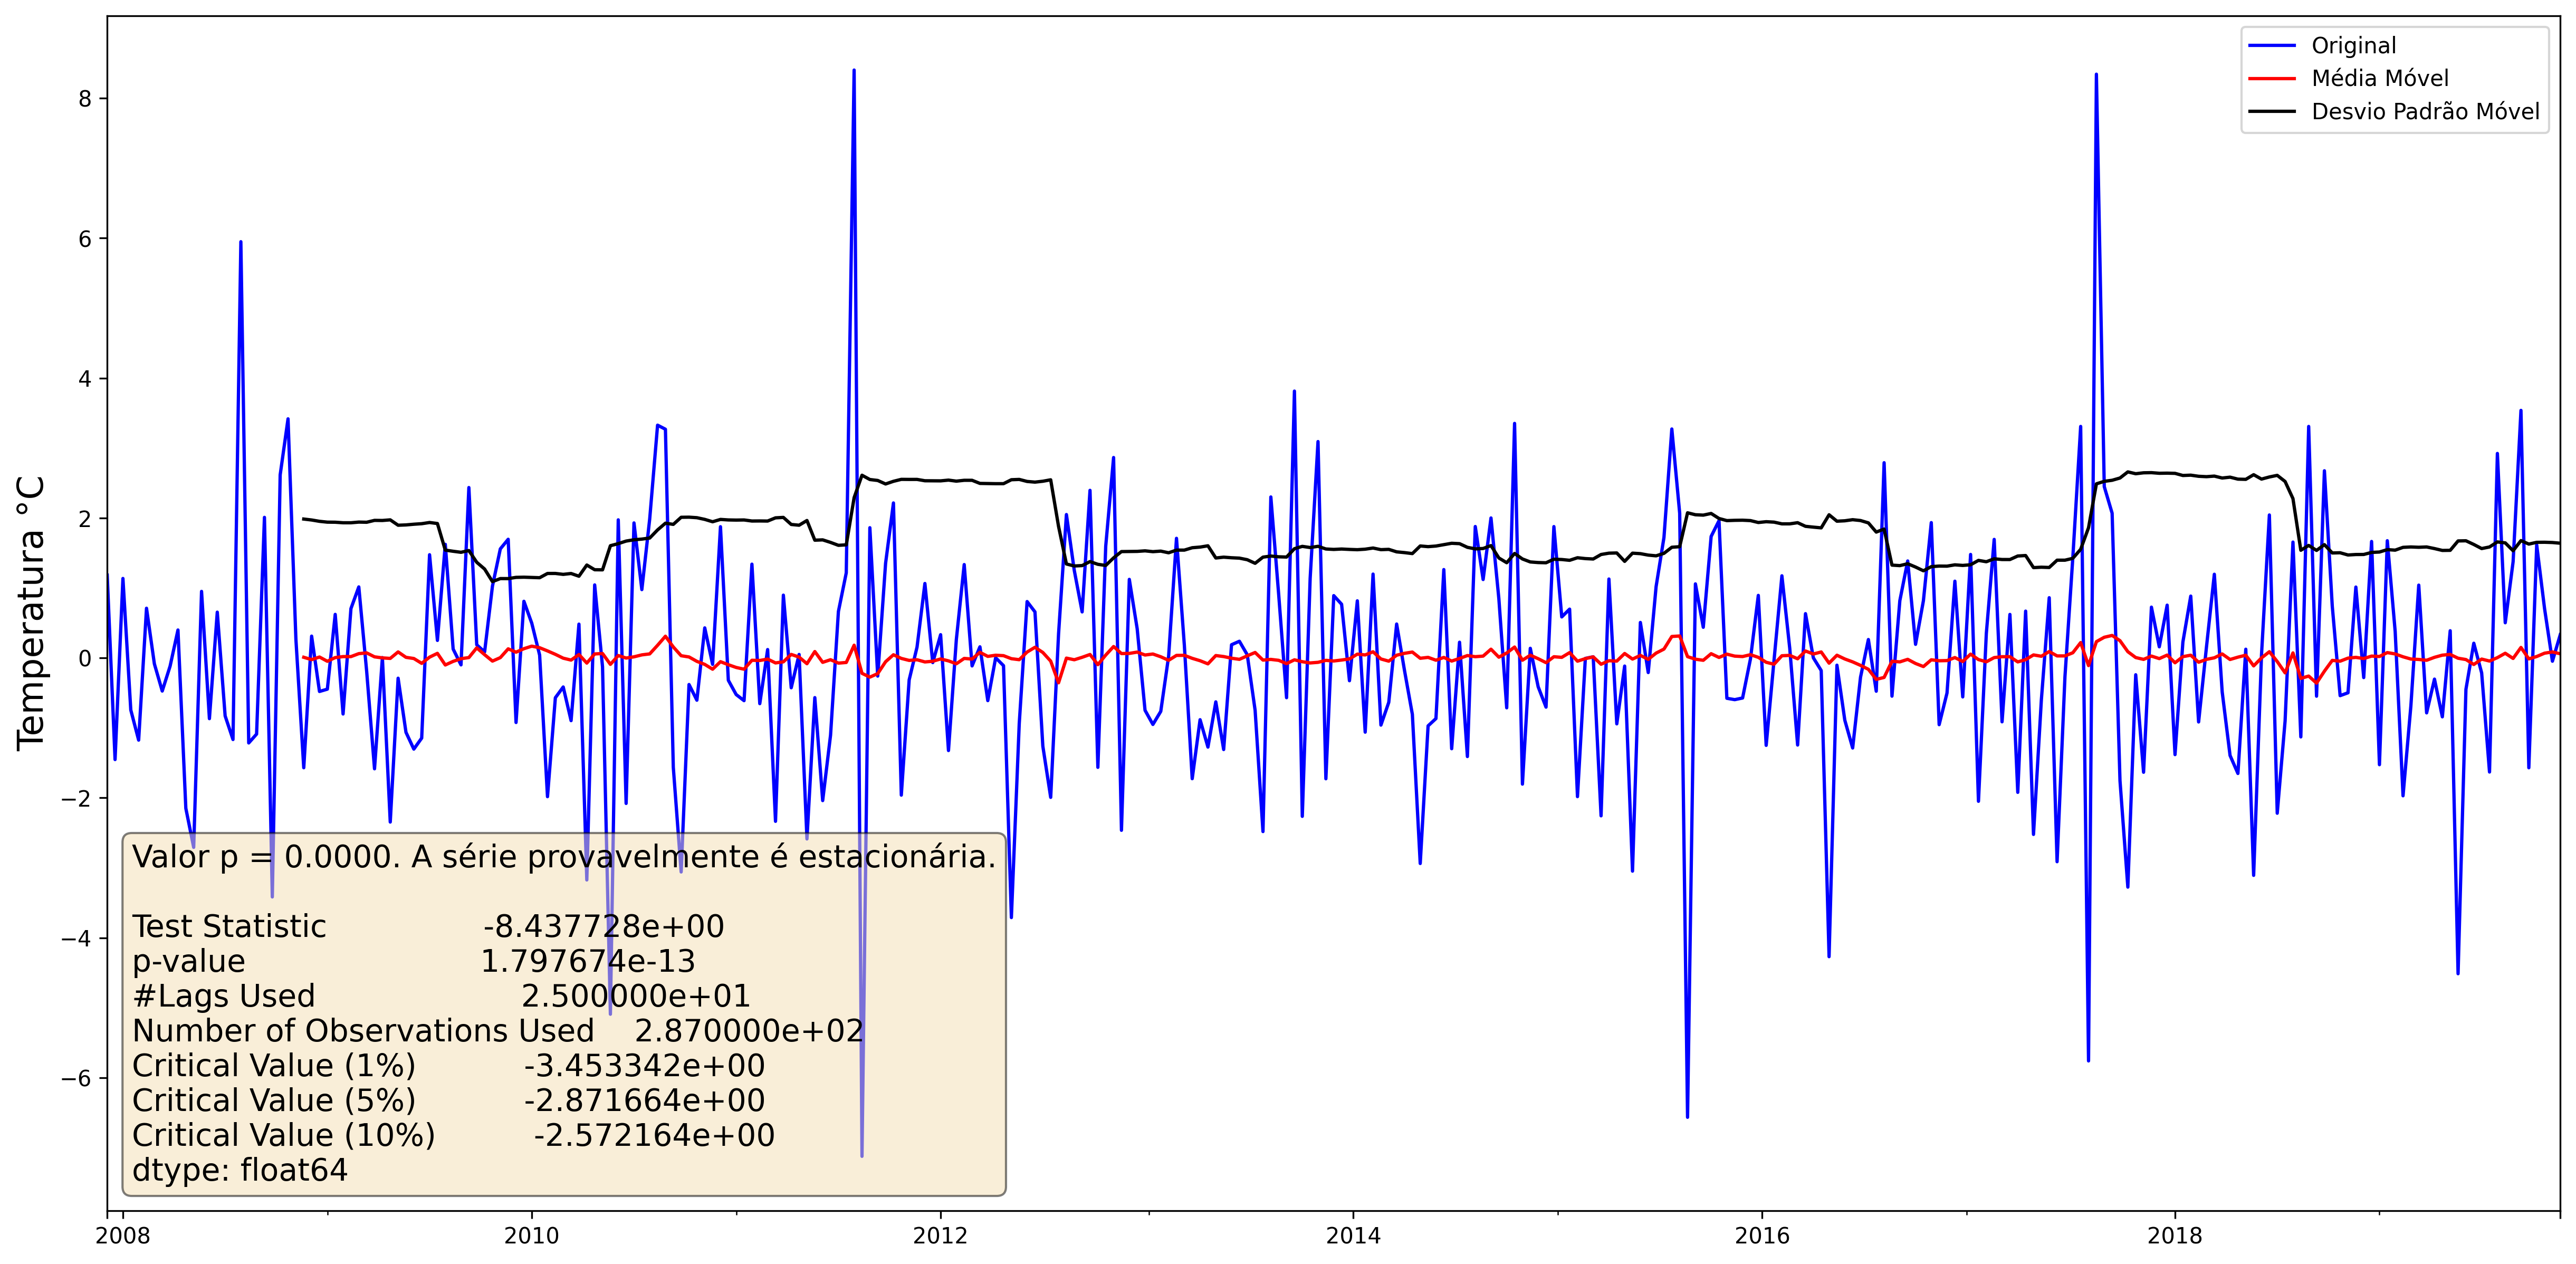
\includegraphics[width=0.9\textwidth]{figuras/dickey_fuller_diff_A736.png}
    \label{fig:estacionalidade_seria_diferenciada_2}
\end{figure}

\begin{figure}[H]
    \centering
    \caption{Teste de estacionalidade da série temporal diferenciada da temperatura do ar para a estação automática localizada no município de Petrolina, no estado de Pernambuco.}
    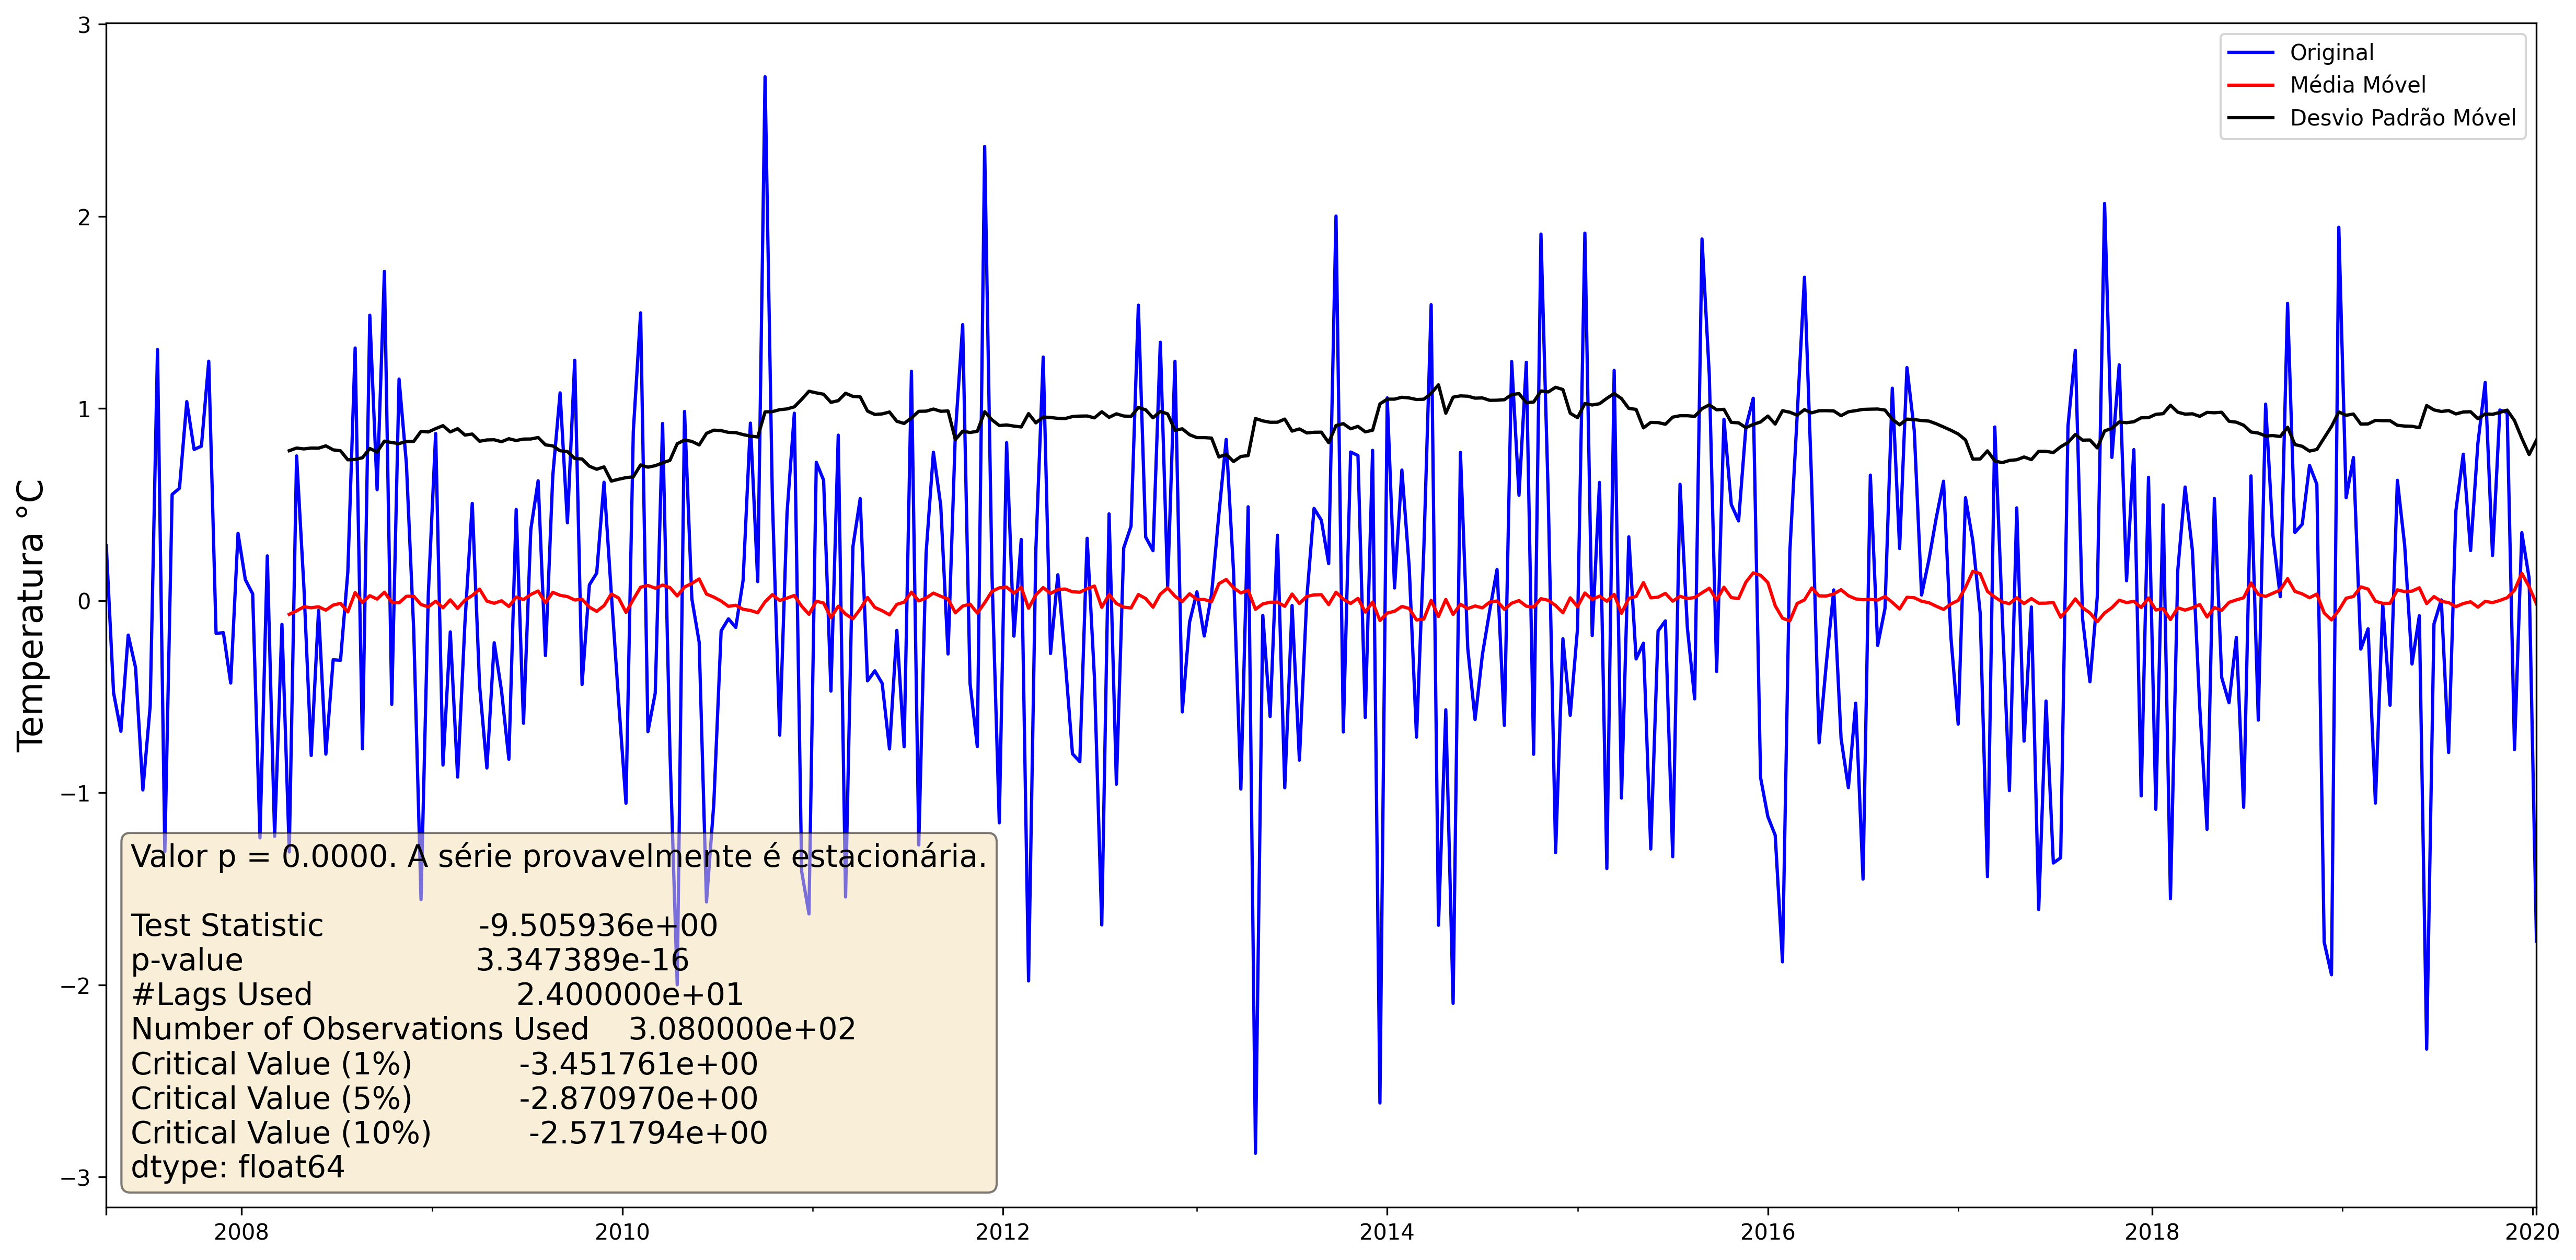
\includegraphics[width=0.9\textwidth]{figuras/dickey_fuller_diff_712f3e11658051636f09732a60fb3c1b.png}
    \label{fig:estacionalidade_seria_diferenciada_3}
\end{figure}

Após a diferenciação, todas as séries ficaram com o valor p abaixo de 0,05 e consequentemente passaram no teste da estacionalidade. Agora será possível parametrizarmos e treinarmos o modelo de previsão ARIMA. 

\subsection{Parametrizando o modelo ARIMA}

Para a parametrização do modelo, utilizamos a abordagem proposta por \citeonline{hyndman2007automatic}. Essa abordagem testa iterativamente um conjunto de parâmetros buscando encontrar a combinação que gera um modelo com o menor valor para a métrica Akaike Information Criterion (AIC) \cite{sakamoto1986akaike}, ou seja, ele busca o melhor modelo ajustado sem ter que testar exaustivamente todas as combinações possíveis. Apesar dessa abordagem buscar o modelo com a melhor combinação de parâmetros, é necessário informar antecipadamente o intervalo de possíveis valores para os parâmetros que ele utilizará para testar os modelos. Apresentamos na Tabela \ref{tab:lista_parametros_arima} a lista dos principais parâmetros que serão ajustados.

\begin{table}[H]
\caption{Parâmetros do modelo que serão ajustados iterativamente.}
\label{tab:lista_parametros_arima}
\begin{adjustbox}{width=\textwidth}
\begin{tabular}{|l|l|}
\hline
\textbf{Nome do Parâmetro} & \textbf{Descrição}\\
\hline
p  & número de time lags do modelo auto-regressivo (AR) \\
\hline
q & ordem do modelo de média-móvel (MA) \\
\hline
d & grau de diferenciação \\
\hline
P & termo auto-regressivo para a parte sazonal \\
\hline
Q & termo da média-móvel para a parte sazonal \\
\hline
D & termo de diferenciação para a parte sazonal \\
\hline
\end{tabular}
\end{adjustbox}
\end{table}

Realizamos a busca pelo melhor modelo para cada uma das 88 estações selecionadas para análise. Para o processamento utilizamos a biblioteca escrita na linguagem Python pmdarima \cite{smith2017pmdarima}, versão 1.7.1. A Figura \ref{fig:parametros_auto_arima} apresenta todos parâmetros utilizados pela biblioteca pmdarima para buscar o melhor modelo para cada uma das estações avaliadas. 

\begin{figure}[H]
\centering
\caption{Parâmetros utilizados na função auto\_arima, da biblioteca pmdarima, para buscar o melhor modelo ajustado.}
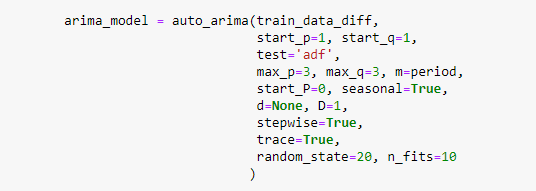
\includegraphics[width=0.9\textwidth]{figuras/parametros_autoarima.png}
\label{fig:parametros_auto_arima}
\end{figure}

\section{Criação do modelo LSTM}

As redes neurais recorrente do tipo Long Short-Term Memory (LSTM) tem a promessa de aprender longas sequências de observações, o que é desejável em nosso caso, já que possuímos algumas estações convencionais com observações que datam do ano 1961, ou seja, 58 anos de observações.  Mas para isso, elas exigem que utilizemos grandes conjuntos de dados de treinamento. Nesta seção,  apresentaremos a arquitetura desenvolvida e os passos executados para realizar as previsões utilizando este modelo. 

\subsection{Conjunto de dados de treinamento, validação e teste}

Para o treinamento e análise da acurácia do modelo, os dados foram separados em três conjuntos distintos, treinamento, validação e teste. Segundo \citeonline{hastie2009elements}, o conjunto de treinamento deve ser usado para ajustar o modelo; o conjunto de validação deve ser usado para estimar o erro da predição do modelo, e o conjunto de teste deve ser utilizado para a avaliação do erro da generalização do modelo final escolhido. 

Para o conjunto de teste, assim como no modelo ARIMA, utilizamos as mesmas 88 estações que selecionamos na Figura \ref{tab:amostra_estacoes} como amostras para a avaliação dos modelos. O conjunto de treinamento e validação geramos a partir das estações restantes, ou seja, de todas as 878 estações, utilizamos as mesmas 88 estações, que foram utilizadas no modelo ARIMA,  para a geração dos dados de teste e as 788 estações restantes utilizamos para o treinamento e validação do modelo LSTM.

O nosso modelo receberá como dado de entrada, chamaremos de X, uma série de observações de temperatura e retornará como previsão, chamaremos aqui de Y, os valores de temperatura média previstos para o próximo ano. Para criarmos um grande conjunto de dados de treinamento, ao invés de dividirmos uma série temporal em um único par (X, Y) utilizando Y como o último ano e X como os dados dos anos anteriores, vamos utilizar aqui deslocamentos de um ano na série para obtermos, de uma única série, múltiplos pares (X, Y). Na Tabela \ref{tab:dados_de_treinament_lstm} apresentamos todos os períodos utilizados para gerar os valores (X, Y) que foram utilizados para treinar o modelo LSTM. 

\begin{table}[H]
\centering
\caption{Quantidade de registros por conjunto de dados obtidos.}
\label{tab:dados_de_treinament_lstm}
\begin{adjustbox}{width=\textwidth}
\begin{tabular}{|l|l|}
\hline
\textbf{Período para obter o dado de entrada (X)} & \textbf{Período para obter a saída esperada (Y)}\\
\hline
todos os dados antes de 01/01/2019  & 01/01/2019 - 31/12/2019 \\
\hline
todos os dados antes de 01/01/2018  & 01/01/2018 - 31/12/2018 \\
\hline
todos os dados antes de 01/01/2017  & 01/01/2017 - 31/12/2017 \\
\hline
todos os dados antes de 01/01/2016  & 01/01/2016 - 31/12/2016 \\
\hline
todos os dados antes de 01/01/2015  & 01/01/2015 - 31/12/2015 \\
\hline
todos os dados antes de 01/01/2014  & 01/01/2014 - 31/12/2014 \\
\hline
todos os dados antes de 01/01/2013  & 01/01/2013 - 31/12/2013 \\
\hline
todos os dados antes de 01/01/2012  & 01/01/2012 - 31/12/2012 \\
\hline
todos os dados antes de 01/01/2011  & 01/01/2011 - 31/12/2011 \\
\hline
todos os dados antes de 01/01/2010  & 01/01/2010 - 31/12/2010 \\
\hline
\end{tabular}
\end{adjustbox}
\end{table}

Após processar todos os períodos, obtivemos 5.137 séries com os valores de entrada (X) e 5.137 séries com os valores esperados (Y). Destas, 75\% dos pares(X, Y) foram alocados no conjunto de treinamento e 25\% foram alocados no conjunto de validação.  


\subsection{Normalização dos dados}

Para normalizar os dados de treinamento, utilizamos a função MinMaxScaler da biblioteca sklearn \cite{pedregosa2011scikit}, própria para aprendizado de máquina. Essa função tem como objetivo mapear os dados a serem normalizados no intervalo [0, 1]. Dessa forma, o maior valor que será normalizado receberá o valor de 1, e o menor, o valor de 0, os valores intermediários serão transformados em números dentro desse intervalo.

\subsection{Modelo LSTM desenvolvido}

Para a construção do modelo, utilizamos a biblioteca TensorFlow, versão 2.3.0. O modelo desenvolvido utiliza duas camadas LSTM, com 128 neurônios do tipo LSTM cada. Como camada de saída utilizamos uma camada densamente conectada com  ativação linear e 26 neurônios, cada neurônio será responsável por prevê um dos 26 períodos de duas semanas que compõe o ano que será previsto pelo modelo. Configuramos o modelo para utilizar o otimizador Adam com taxa de aprendizado de 0,001. Como função de perda utilizamos o Mean Squared Error (MSE) e como métrica de avaliação o Mean Absolute Error (MAE). A Figura \ref{fig:modelo_lstm} ilustra o modelo completo desenvolvido. 

\begin{figure}[H]
\centering
\caption{Arquitetura LSTM desenvolvida.}
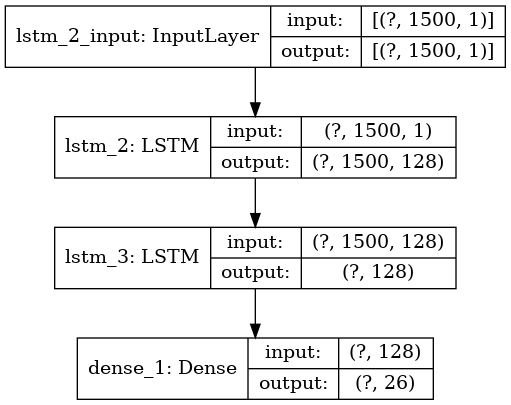
\includegraphics[width=0.5\textwidth]{figuras/lstm_model.png}
\label{fig:modelo_lstm}
\end{figure}

Para o treinamento do modelo, utilizamos lotes com 128 itens, treinando por 44 épocas. Utilizamos o \textit{callback} EarlyStopping do Keras para realizar uma parada precoce no treinamento com o objetivo de evitar ajustes excessivos no modelo. A Figura \ref{fig:perda_modelo} ilustra a perda do modelo ao longo do processo de treinamento. 

\begin{figure}[H]
\centering
\caption{Perda do modelo durante o processo de treinamento.}
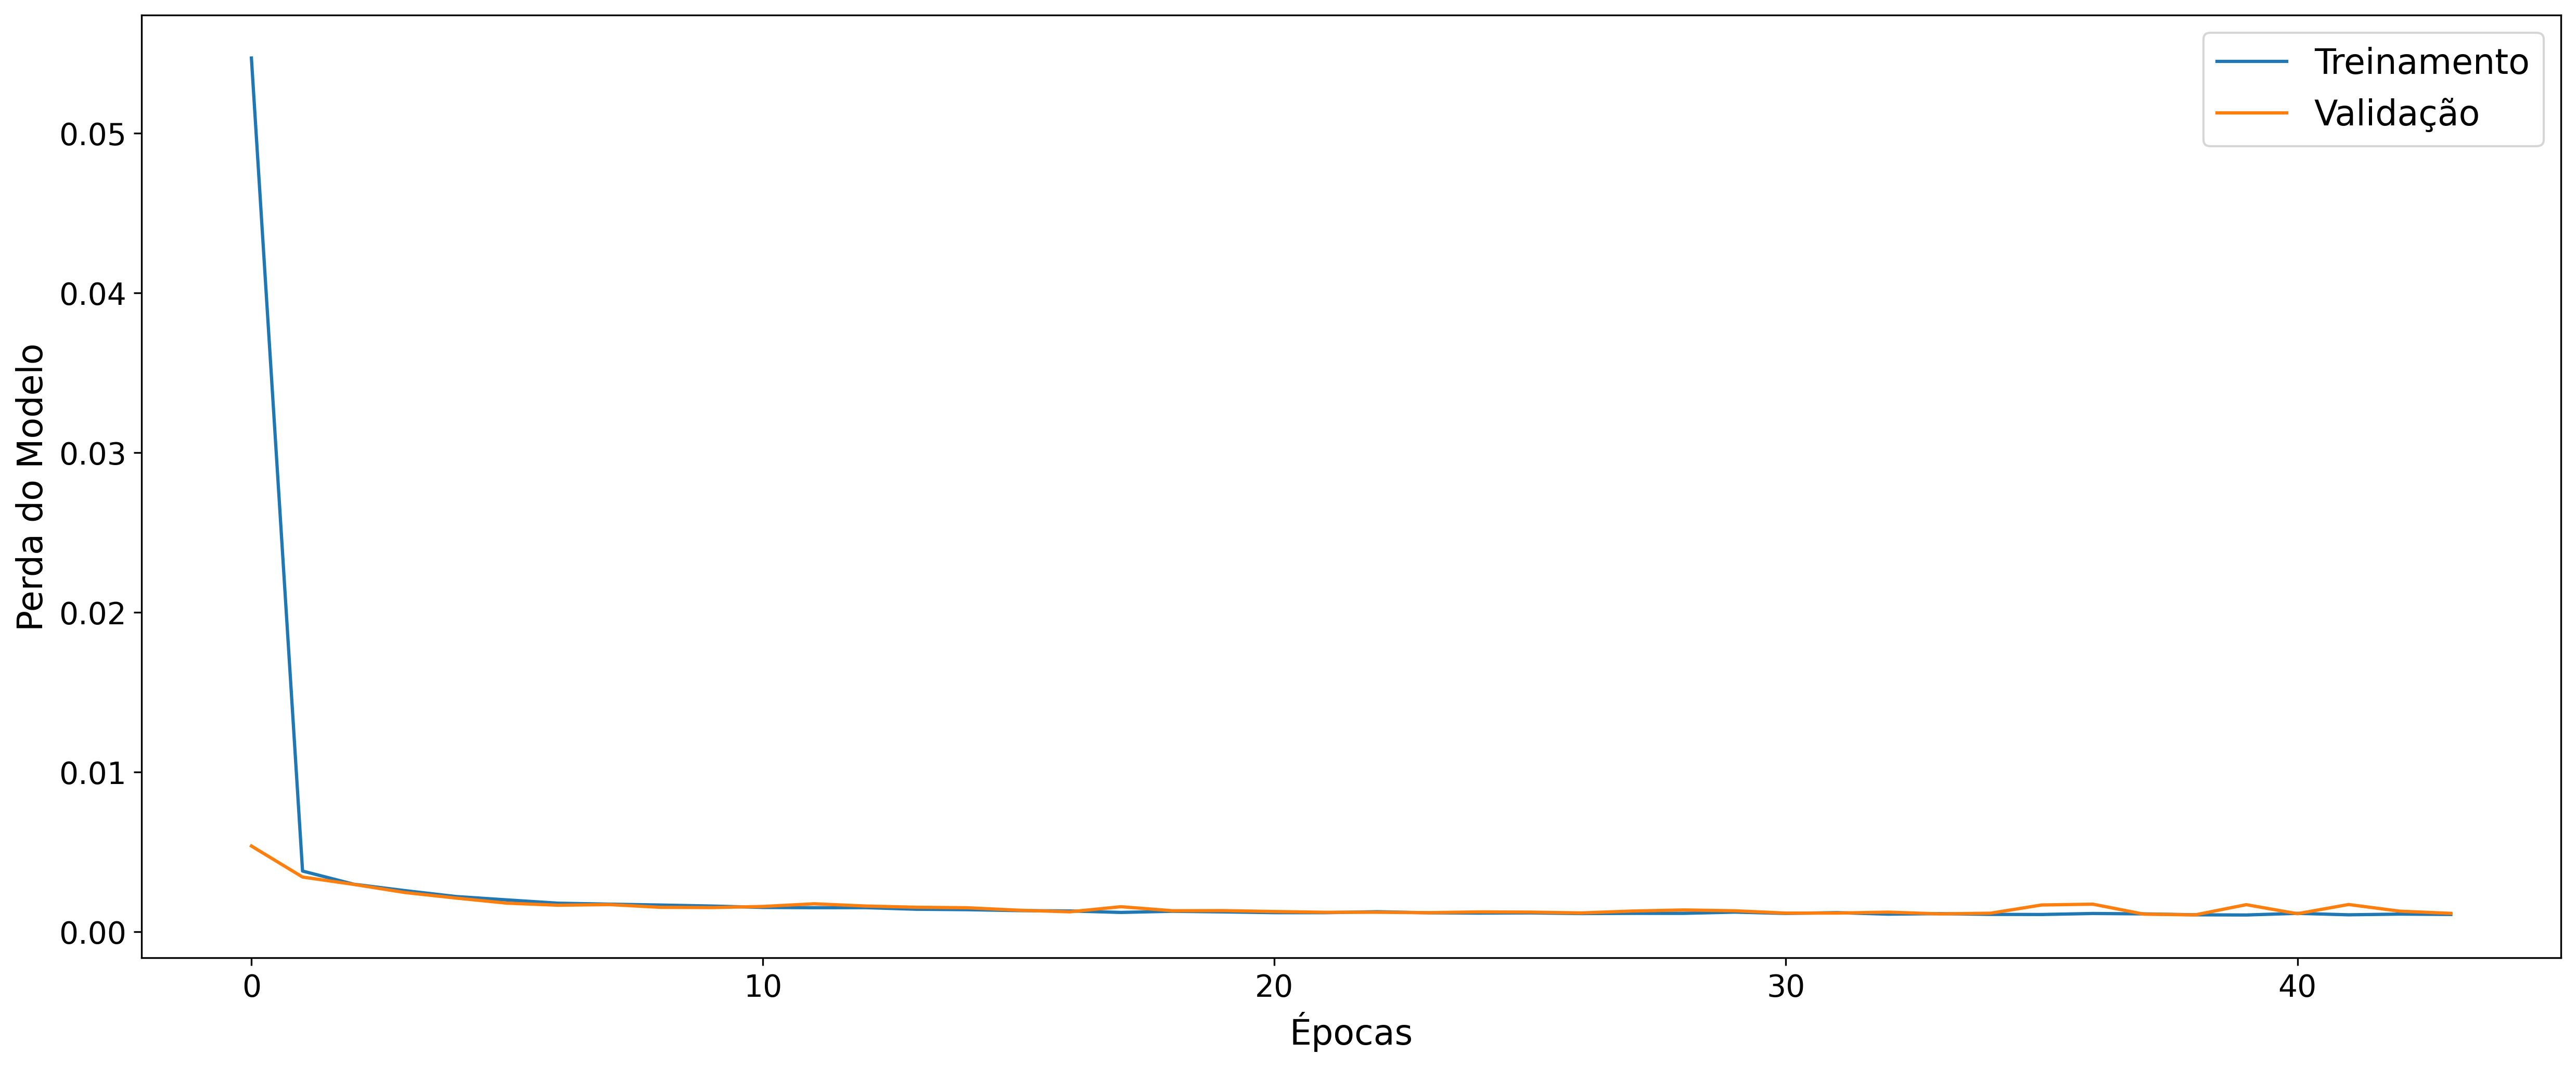
\includegraphics[width=\textwidth]{figuras/grafico_de_perda.png}
\label{fig:perda_modelo}
\end{figure}

\renewcommand{\cleardoublepage}{}
\renewcommand{\clearpage}{}
\vspace{5mm}